\chapter[Polarized $^3$He Target]{Polarized $^3$He Target
\footnote{
  $CVS~revision~ $Id: pol-he3.tex,v 1.32 2008/09/16 19:50:55 jpchen Exp $ $
}
\footnote{Authors: Revised by: T. Averett, J. P. Chen, C. Dutta, J. Katich,
Y. Qiang. earlier versions: 
T. Black, J. P. Chen, P. Chevtsov, H. Gao, 
O. Hansen, S. Incerti, S. Jensen, M. G. Jones, K. Kramer, M. Liang, 
N. Liyanange, K. McCormick, Z.-E. Meziani, X. Zheng.
\email{jpchen@jlab.org}}
}

\section{General Description}
\label{sec:target-he3-general}
\subsection{Physics Principle}

This target system provides a high-density 
($\approx 2.5\times 10^{20}$ nuclei/cm$^3$)
polarized $^3$He gas target for spin physics experiments. 

The target employs the so-called spin-exchange technique.
In the traditional spin--exchange technique $^3$He is polarized in 
a two-step process.
First, rubidium vapor is polarized by optical pumping with
circularly polarized 795~nm laser light. Second, the polarization
of the Rb atoms is transferred to the $^3$He nucleus in spin-exchange
collisions, in which $^3$He nuclei are polarized via the hyperfine interaction.
Recently,a noval technique of hybrid pumping has been used.  
In addition to the direct spin exchange, it also happens indirectly for the 
hybrid Rb-K cells: spin-excahnge first happens between rubidium and potassium atoms 
(very fast) and 
then between potassium atoms and $^3$He nuclei, which is more efficient 
than the direct Rb-$^3$He spin exchange.
The target cell contains high pressure $^3$He gas and a small amount of
vapor of Rb-K mixture. 
In addition, it
also contains a small amount of nitrogen to increase the
pumping efficiency.

\subsection{Apparatus}

High power infrared (795 nm) diode lasers (about 100\,W) provide an intense 
monochromatic
light beam for optical pumping. 
The lasers are housed in a laser room
outside the hall next to the counting house. Laser light goes to the hall 
through an optical fiber system.  An overview of a
typical arrangement of the target components in the Hall is shown in
Fig.~\ref{fig:overview}.

\begin{figure}[p]
\begin{center}
%\centerline{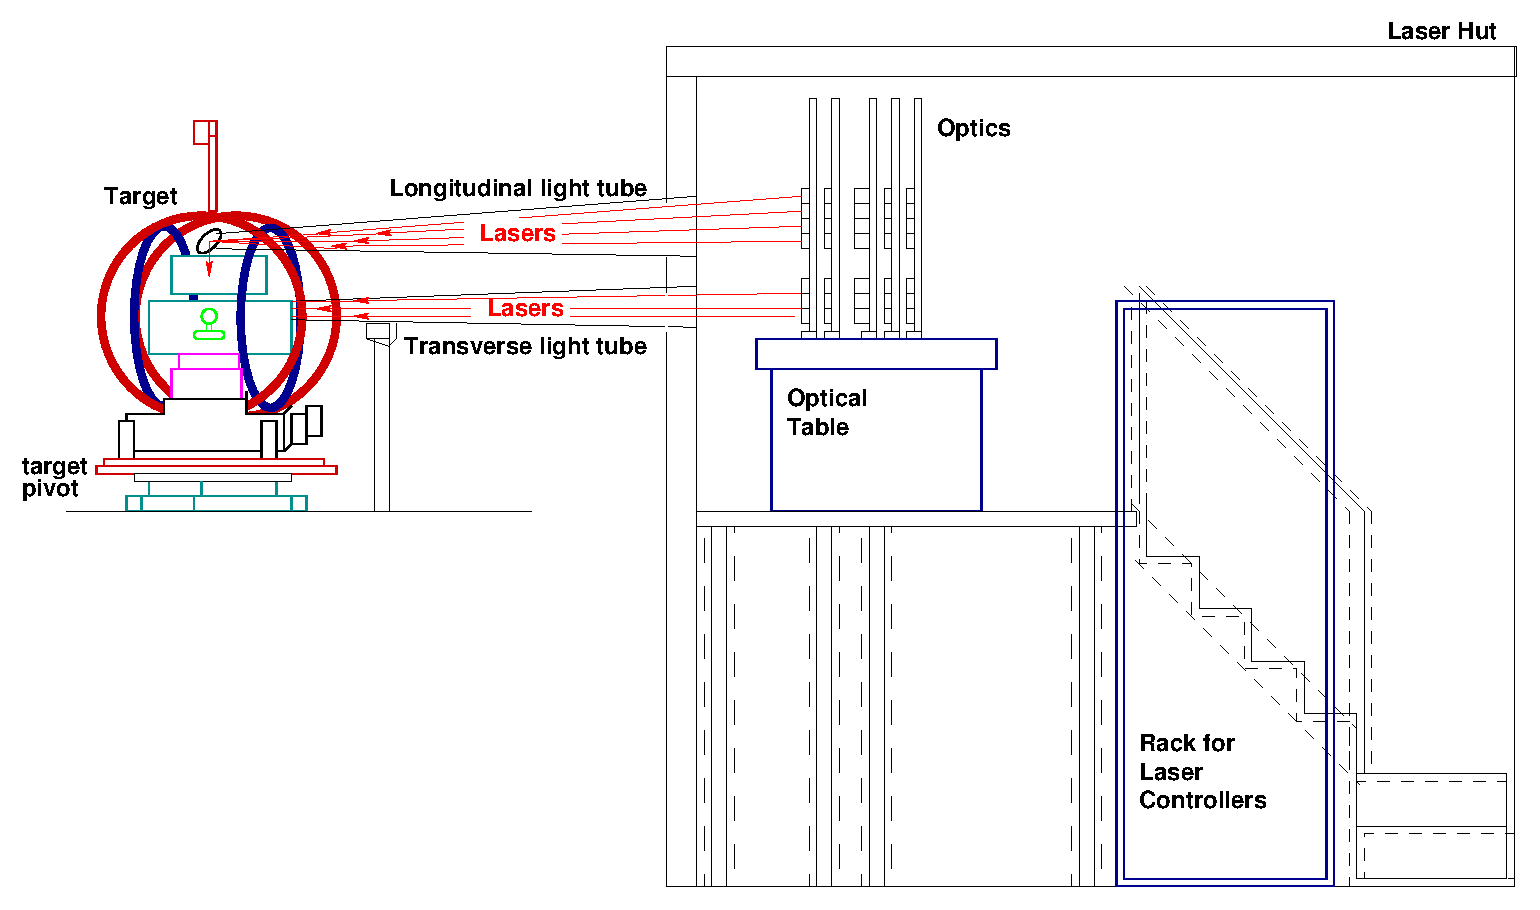
\includegraphics[scale=0.6]{overview_may23}}
\centerline{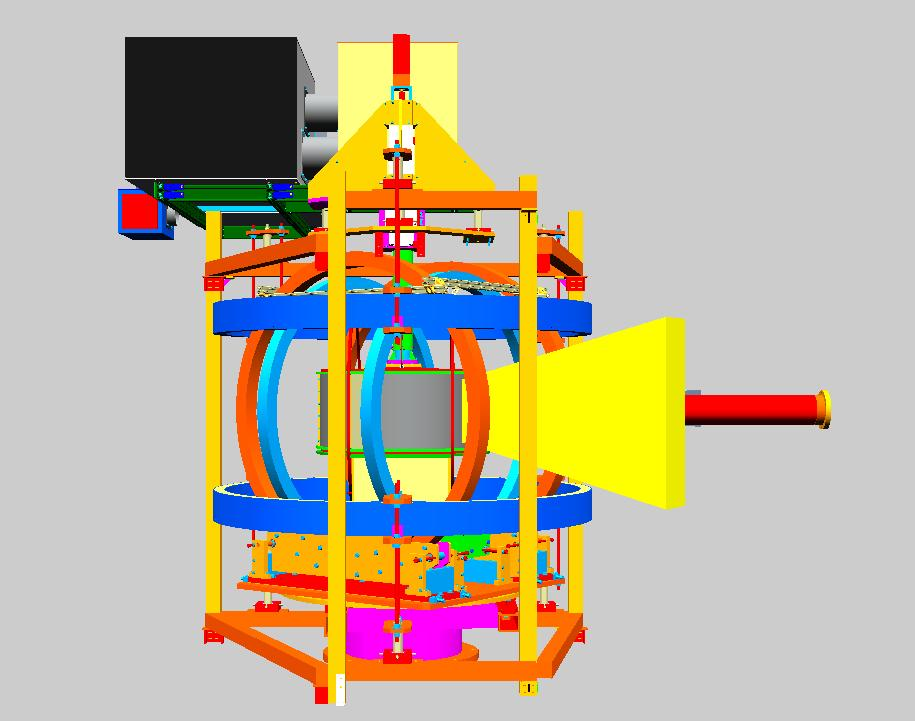
\includegraphics[scale=0.6]{OverView}}
\end{center}
\caption[Overview of the polarized $^3$He target setup]%
{Overview of the target setup. Shown are the laser
beam pipes covering the laser beam line on top of the target area,
and the three sets of Helmholtz coils with the support sub-assembly. }
\label{fig:overview}
\end{figure}

The polarized target comprises several
components beyond its target cell (see Fig.~\ref{fig:overview})
related to its operation, they are in subsection:

\begin{enumerate}

\item 
Three sets of orthogonal Helmholtz coils provide the target spins with a
holding magnetic field 
of few tens of Gauss as well as define the orientation of the
polarization in any required 
direction. The set of vertical coils
is a new addition and will be used for the first
time for the transversity experiment\cite{E06010}.

\item
Two pairs of RF coils which allow for the measurement of the target
polarization
using the Adiabatic Fast Passage (AFP) technique and the Electron
Paramagnetic 
Resonance (EPR) technique, as well as a way to flip target spin direction.

\item
A multi-purpose enclosure which is part of the laser light enclosure and
provides a
containment of the target cell in case of explosion. It also provides a
containment volume for the
$^4$He gas to cool the target windows with cooling jets, minimizing the
radiation length crossed  by the electron beam. 

\item 
An oven with all its related components for providing the necessary
temperature to the  pumping cell in order to bring Rb and K
in their vapor phase 
and control their number densities. 

\item 
A target ladder subassembly which supports a target cell,  a reference
cell, (which can be filled with Hydrogen, $^3$He or Nitrogen gas 
with pressure
up to 10 atmospheres for calibration or to study dilution, density or 
background), a multi-foil $^{12}$C optics target, a
BeO beam viewer and an oven. It also includes a full mechanism
for positioning the targets 
and bears the target cell viewing mirrors and the optical beam line
mirrors. 

\item 
A laser and optical fiber system in the laser room bring 
up to fifteen laser beams, each from 
a 30-Watt diode laser, to the hall. 
These laser beam lines are used for optical
pumping of the rubidium-potassium alkali atoms in three different directions:
along the electron beam (longitudinal), perpendicular to the electron
beam line but on the horizontal plane (transverse) and the vertical. They can 
also be re-directed to any direction as needed.
\end{enumerate} 


\subsection{Control System}

The control (including monitoring and measurement) system for
the target Helmholtz coil magnet power supplies, the NMR polarimetry
and the EPR polarimetry is based on the LabView system on a PC.
The control system for the target vertical motion, the lasers,
the oven heater, and temperature and pressure monitoring
runs under the EPICS~\cite{EPICSwww} environment utilizing
 an IOC in a VME crate. The LabView system 
records data on disk and communicates with the 
EPICS system through the network. Information from the EPICS IOC is logged 
on disk and selected information passed to the event data stream.

\infolevtwo{
%=============================================
%\chapter
\section{Operation Overview}
\label{sec:Opover}

In normal operation the target will be under one of the following
situations described below.

\begin{safetyen}{10}{5}

\begin{enumerate}

\item 
The target is in ``beam position'', the fast raster set to a
nominal 4 mm $\times$ 4 mm area coverage and the experiment is
running to collect physics data. In this configuration the monitoring
of the target consists of reading a set of temperatures of the pumping
cell, target cell and reference cell. The temperature in the pumping
cell provides feedback for the temperature controller.  A spectral-analyzer
is monitoring the laser wavelength and the relative intensity.
All interlocks of electron beam and laser beam should be on.

\item 
The beam is turned off and the target is moved to ``Pickup Coil Position''
(polarized $^3$He target in a position
between the NMR pickup coils) and a polarization measurement is
performed using the NMR (AFP) method.  The laser beam will be stopped
first. If the polarization is in the transverse mode, 
a rotation of the polarization to the longitudinal direction is
performed (procedure described in Section~\ref{sec:nmr}).  Once the
measurement is completed the target cell will be moved back to the ``beam
position''. If the next running is in transverse mode, a rotation of
the polarization to the transverse direction is performed.
The laser beam will be turned on. The beam interlock is
reset and the fast raster enabled before turning the beam back on
target. The physics data taking should resume. 

\item 
The ``Polarized $^3$He Target'' is either in ``beam position'' or in ``pick-up
coil position''.  The data taking is stopped and the 
beam is turned off. An EPR measurement is performed (procedure described in 
Section~\ref{sec:epr}). After the measurement
is completed and the fast raster enabled, the beam is put back on and
data taking resumes.

\item 
The ``BeO Target'' is moved to ``beam position''.
The electron beam current lowered (to $<~5~\mu$A with raster-off) 
as not to damage the 
BeO target.  The monitoring of the beam
position is performed by looking at the TV monitor which displays the
view of the target.

\item 
The multi-foil $^{12}$C ``Optics Target'' is in ``beam position''. Data on the optics
target are taken for spectrometer optics study or detector calibration.
Since the BeO and the optics target are in beam at the same time, the above 
two measurements are often performed at the same time.

\item
The ``hole'' target is in ``beam position''. The ``hole'' target is
a signle $^{12}$C foil with a 1 mm square hole at the center. It is used for
center the beam with respect to the target ladder.  

\item 
The target ladder ``Empty Target''
frame is moved to ``beam position'' whenever
beam tuning is performed, and when checking for possible beam halo
background.

\item  
The ``Reference Cell Target'' is in ``beam position'' with the beam fast
raster on and data on the reference cell are taken for calibration.


\end{enumerate}

\end{safetyen}
%=============================
%\chapter
\section{Laser System}
\label{sec:lasers}

The laser system provides 795\,nm circularly polarized light for optical
pumping of the target. The light is generated by several solid-state
diode lasers, which are located in a laser room outside the hall.
Each laser emits roughly 30W of
power and is transported into the hall with an 75 meter long optical 
fiber. Up to five laser beams are combined to one through a 5-to-1 combiner.
It is then polarized by passing through a polarizer 
(beam splitter) followed by standard $\lambda/4$ waveplates.  
\begin{safetyen}{10}{5}
  Because of the invisibility and high intensity of the
laser beam, the lasers present a significant safety hazard.
\end{safetyen}
The system generates three independent laser beams for optical
pumping of three different target spin directions: parallel,
perpendicular, or vertical to the electron beam.  In the standard
configuration, up to five lasers are used for each direction.  
Further, the laser polarization direction can be reversed 
by rotating the $\lambda/4$ waveplates by 90 degrees.

%-----------------------
\subsection{Laser Room \& Beam Path}
\label{sec:las}

To protect the lasers from radiation damage due to the electron beam
and shield personnel from accidental exposure to hazardous laser
light, all laser systems are located in a laser room outside the hall.

%Laser beams are trasported into the hall through long optical fibers.
%Fig. \ref{overview} shows the overview of the laser optics system.

%\begin{figure}
%\begin{center}
%\centerline{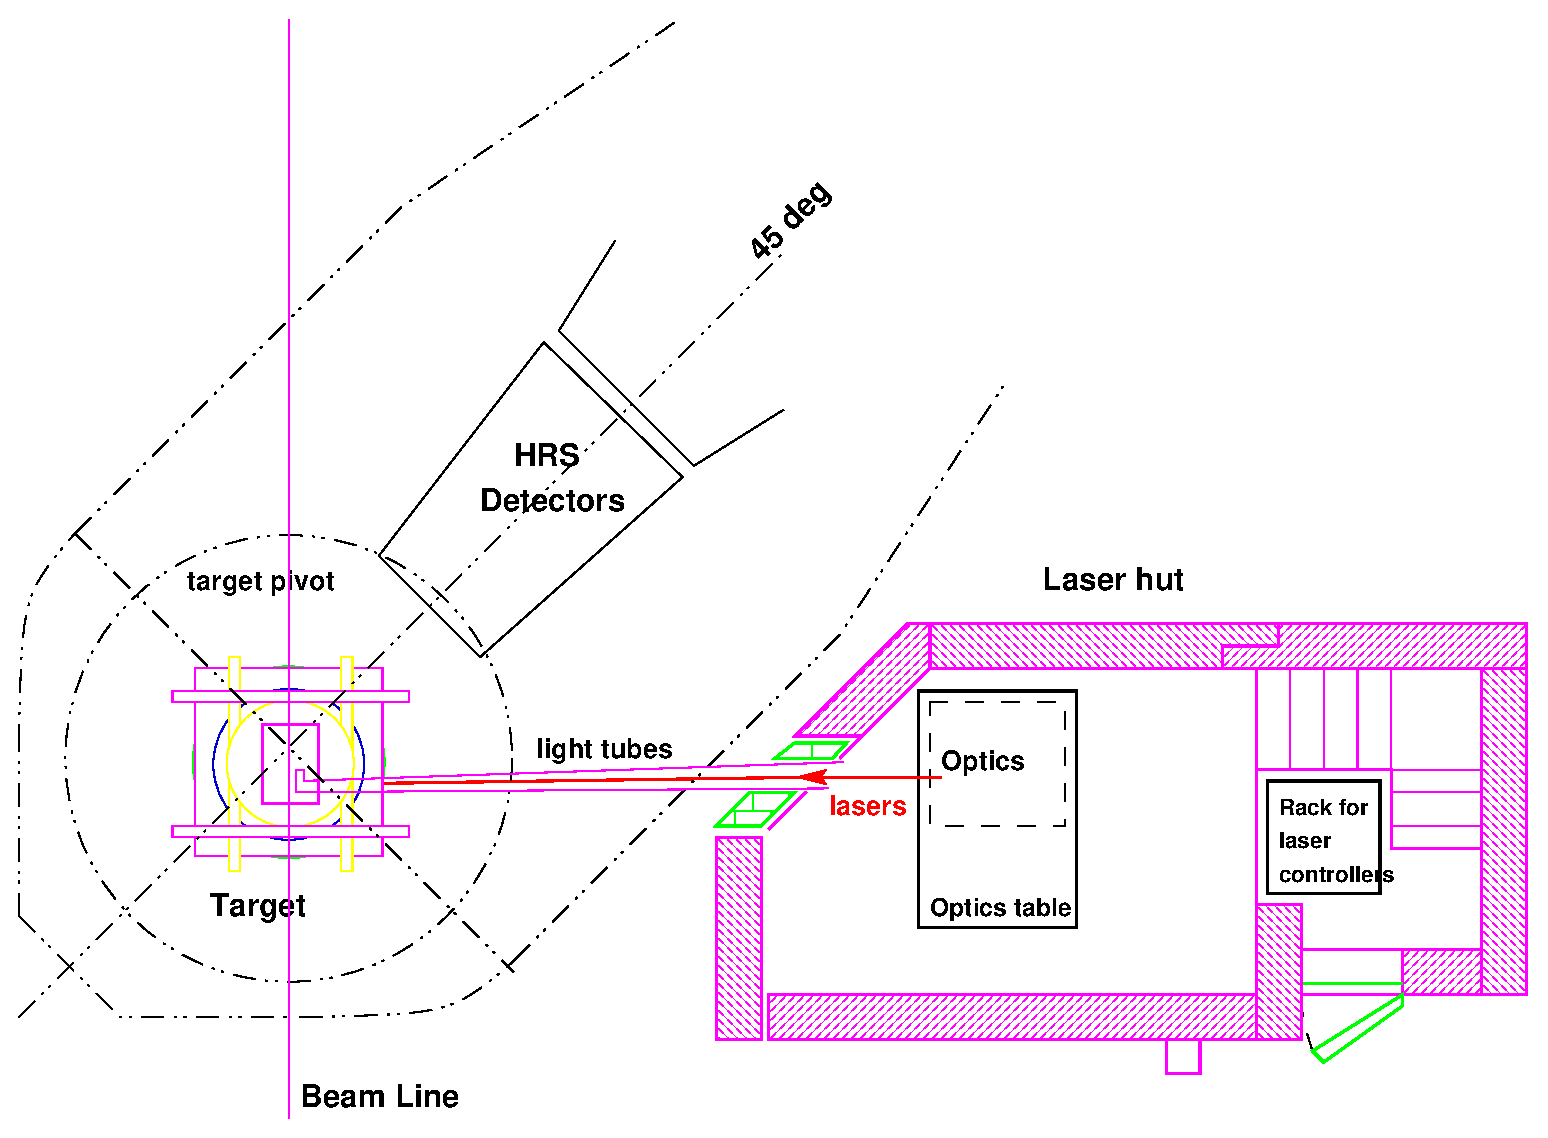
\includegraphics[scale=0.6]{topoverv_may23}}
%\caption[A topview of the laser hut]{ A topview of the laser hut shows the location
%of the interlocked door as well as the position of the laser table where
%all lasers and optics will be set up.}
%\label{fig:overview}
%\end{center}
%\end{figure}

%Inside the laser hut, an optical table with an anodized aluminum top
%supports all optics. The setup of the
%polarizing optics is shown in Fig.~\ref{fig:laser_setup}. 

Up to 15 infrared diode lasers (five for each pumping direction) and 
the related interlock control box are located on two 19" racks in the laser room.
Light is guided out of each laser and 
goes into the hall via an optical fiber.  
Five beams combined to one with a 5-to-1 combiner. 
The combined beam is focused by two 2" diameter convex lens then 
divided by a polarizing
beam splitter cube into two linearly polarized rays.  Because the
laser light is initially unpolarized, both the direct and the split
beam carry approximately half the power. To utilize the full laser
power it is necessary to combine both beams and focus them onto the
optical pumping cell.  This is accomplished as follows:

The direct beam is reflected by a 3" diameter dielectric mirror which
can be adjusted to steer it towards the pumping cell.  The split beam
passes through a $\lambda/4$ waveplate, is reflected by a 2" diameter
dielectric mirror, and passes through the $\lambda/4$ waveplate again.  The 
fast and slow axes of this $\lambda/4$ waveplate should be oriented at an 
angle of 45$^\circ$ to the horizontal or vertical direction.  The
linear polarization of this beam is thus rotated by 90$^\circ$, and is
able to pass through the beamsplitter, essentially without
reflection.  The second passing through the splitter is necessary to
achieve a very high degree of linear polarization for the split beam
since the splitter only gives high polarization for direct beam 
($T_P>95$\%,$R_S>99.8$\%).

Now both beams from each laser have identical linear
polarizations.  Each passes through a $\lambda$/4 waveplate that
transforms its polarization from linear to circular.  The orientation of 
each $\lambda$/4 waveplate is shown in Fig.~\ref{fig:laser_setup}, note that 
all $\lambda$/4 waveplates should have the same orientation.

The resulting beams are reflected twice by a
pair of adjustable 6" diameter mirrors mounted on top or
next to the target pumping chamber. These mirrors can be
standard dielectric ones since they will be in a
polarization-preserving compensating configuration (one mirror rotated
by 90$^\circ$ with respect to the other). 
The laser beams are carefully aligned to coincide on the pumping chamber 
of the cell.  They enter the target chamber via transparent
windows on the oven wall.
  

\begin{figure}
\begin{center}
\centerline{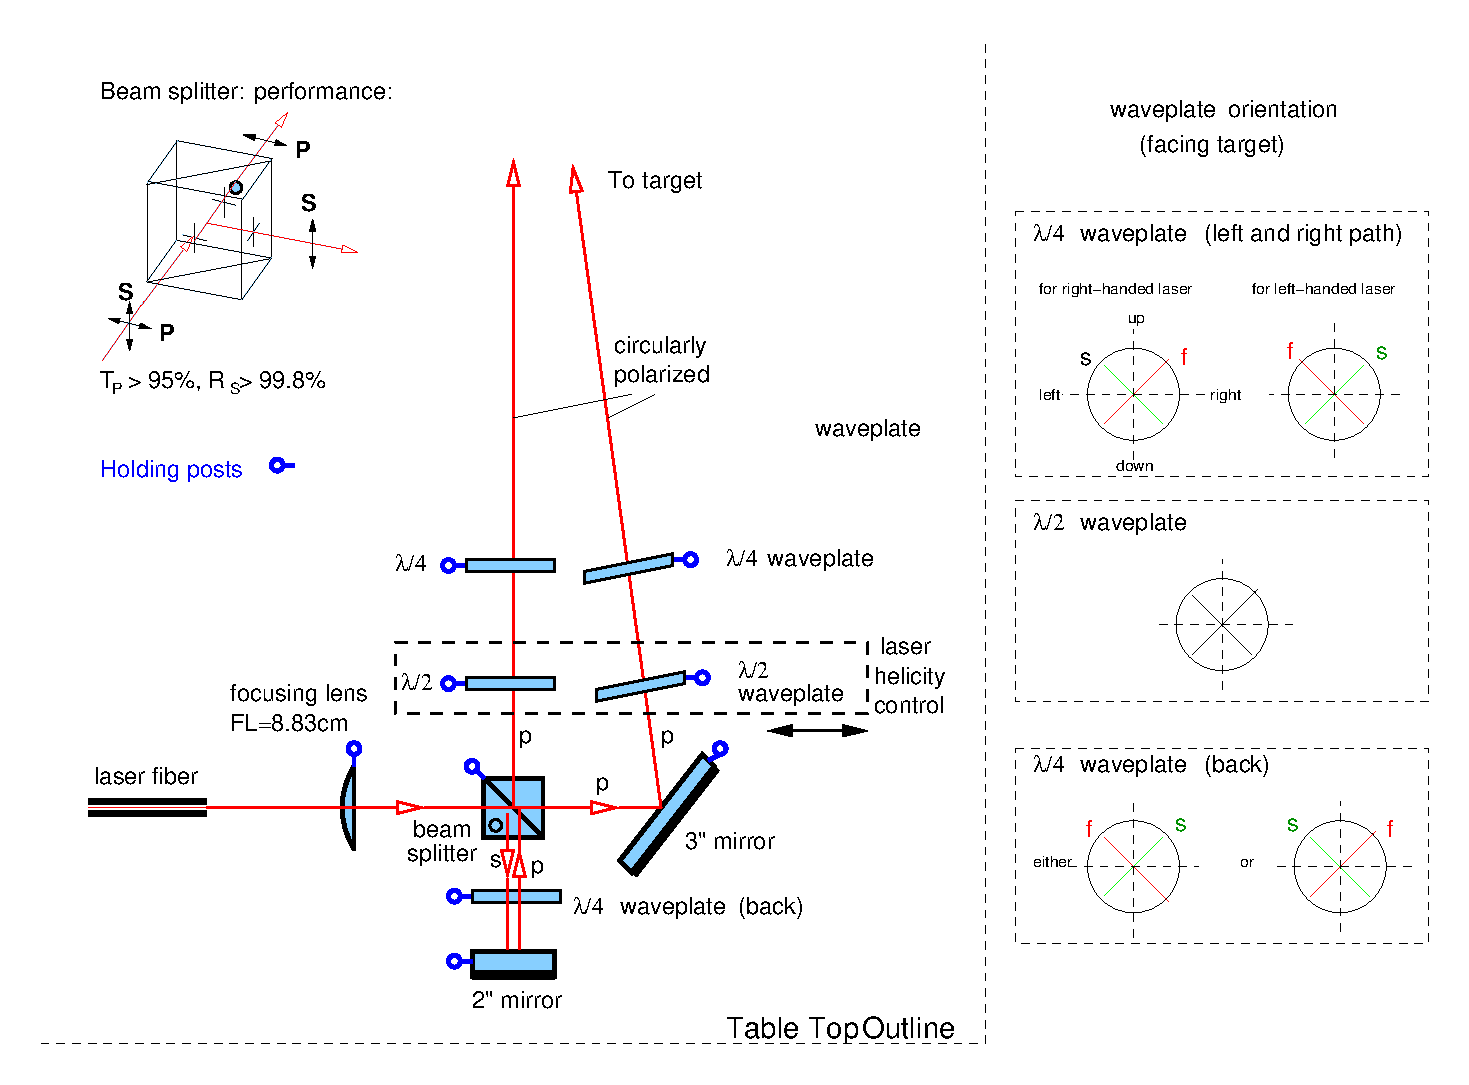
\includegraphics[scale=0.8, angle=90]{laser_setup}}
\end{center}
\caption[Top view of the optics setup]%
{Top view of the optics setup.}
\label{fig:laser_setup}
\end{figure}

Under normal conditions, laser light
will be mostly absorbed by the rubidium in pumping cell.
There are additional windows on the oven to allow lights to be
collected for the EPR measurement and for spectral-analyzer to monitor
laser spectrum and intensity.  
For the ERP measurement, light is focused by two lenses (mounted on the oven) 
into an optical fiber to be transported to 
the EPR photodiode which is located behind a shielding wall.
At the meantime some light will be viewed 
by the spectral-analyzer through an optical fiber.

The laser beam line is
protected by beam pipes that extend from the laser room to the target
area. A laser enclosure with interlock covers the laser optics system and 
the target. It is important to point out that the complete laser beam lines 
and optics system are fully enclosed with laser intrelock system from the 
rest of the hall.

\begin{safetyen}{10}{5}
The entire laser room is a laser controlled area that requires special
safety precautions (see Section 13 and Appendix A).
\end{safetyen}

%-----------------------
\subsection{Diode Lasers \& Controls}

The laser light for experiments is provided by multi (up to 15) 30 Watt, 795
nm solid-state diode lasers.  The primary lasers used during the
experiment are made by Coherent Semiconductor Inc. 
The diode lasers consist of a main enclosure which contains the diode,
power supplies, fans and control systems for the laser.  The laser
light from the diode is sent into a flexible optical fiber which
extends out of the main enclosure and goes into Hall A. 
The fiber is 75m long in a stainless steel jacket.

The lasers operate at diode temperature from $15^{\circ}$ C to
$26.5^{\circ}$ C depending on the system.  They are run at output
power of 30 Watts which uses an operating current of 35-40 Amps.  The
output laser light has a central wavelength of 795 nm with a spectral
width of less than 2 nm. The fiber diamter is 800 microns.  The beam
divergence is $< 0.20$ N.A.

The lasers have a local control system, which is integrated into the
main enclosure.  The local control allows adjustments in operating
current (and therefore the laser power) and diode temperature (and
therefore the wavelength within a small range).

During the experiment the lasers will be controlled remotely through
 EPICS.  The lasers have a serial IO port on the back of the main
 enclosure which is connected to a VME RS-232 port.  There is an
 MEDM~\cite{MEDMwww} GUI interface for each of the lasers, which
 allows remote control and monitoring of current and temperature as
 well as being able to turn each laser on and off.


%-----------------------
\subsection{Alignment}

\noindent
{\bf{Basic procedure for laser alignment}}


\begin{enumerate} \setlength{\parskip}{0ex}
\item Set the height of the diode laser, the center of the polarizing
  cube (beam splitter), the two-inch mirror, the quarter wave plates, 
  the lens, and the three-inch mirror to be at the same height.
\item Viewing along the direction of the cube, the mirror and the wave 
  plates, you should be able to see the target.  Here target refers to
  the 6" mirror on top of the oven.  
 \item Place diode alignment laser such that it passes through the center
  of the polarizing cube and the center of the target.
\item Rotate the cube and change the angle such that the back reflection
  hits the alignment laser and such that the reflection hits the diode
  laser simultaneously.
\item Place the two focusing lens in its mount with the flat side away
  from the diode laser. Adjust them so that the back reflection goes back 
  on itself.
\item Turn the diode laser on at LOW POWER.
\item Adjust the head of the diode laser such that the light goes
  through the center of the lens.
\item Rotate the cube mount such that the light passes through the
  center. Be sure that the cube is mounted so that the light enters 
  the marked side and is reflected towards the two-inch mirror.
\item Turn off the diode laser.
\item Place the two-inch mirror into its mount and move such that the
  alignment laser hits the center.
\item Place a quarter wave plate between the cube and the two-inch
  mirror.
\item Turn the laser on at LOW POWER.
\item Adjust the position of quarter wave plate so that the laser passes through the
  center.
\item Adjust the two-inch mirror so that the reflected light hits 
  the target.
\item If you know the axises of quarter wave plate, rotate it according to 
      Fig.~\ref{fig:laser_setup}.  If not, 
\begin{itemize}
\item Rotate the quarter wave plate so that the light which passes
  through the cube from the two-inch mirror is a minimum.
\item Rotate the quarter wave plate forty-five degrees.
\end{itemize}
\item Adjust the two-inch mirror so that the light hits the target.
\item Check to see where the back reflection of the diode is hitting. It
  should be near the head of the diode laser but not directly on top of
  it. If it is then rotate the cube slightly and realign the two-inch
  mirror. Repeat if necessary.  It is important to keep the back reflection
  away from the fiber since a small amount of back reflected laser could reach 
  the diode through fiber and will damage the laser.
\item Place the three-inch mirror in its mount.
\item Check to see that the diode light is hitting the mirror.
\item Adjust the three-inch mirror so that the light is hitting the
  target.
\item Center a quarter wave plate in the path of each beam.
\item If you know the axises of quarter wave plate, rotate it according to 
      Fig.~\ref{fig:laser_setup}.  If not, you need to do bench test first to 
      find the axises of each quarter wave plate.
\item Repeat for all beams heading towards the target.
\item Be sure that the helicity of each beam line is the same.
\item Place the half wave plates in mounts, adjust the position of the post 
      and the mounts such that all either (or six) laser beams are able to 
      hit the center of the corresponding half wave plates simutanuously.
\item If you know the axises of half wave plate, rotate each one according 
      to Fig.~\ref{fig:laser_setup}. If not, you need to do bench test first to 
      find the axises of each half wave plate.
\end{enumerate}

\medskip
\noindent
{\bf{Testing quarter wave plates}}

\begin{itemize}
\item Find the direction of the axes:

\begin{enumerate}
\item Use the laser beam which passes through the polarizing cube (beam splitter).
\item Place the unknown wave plate in the beam.
\item Place a polarizing cube after the unknown wave plate.
\item Place a power meter perpendicular to the polarizing cube such that it
      measures the power of reflected light. 
\item Rotate the unknown wave plate such that the reflected light coming
  from the second cube is at a minimum.
\item Now one of the axes is in horizontal direction and the other is in
      vertical direction.
\end{enumerate}

\item Make sure the axes of all quarter wave plates are identical (either fast or slow):

\begin{enumerate}
\item Use the laser beam which passes through the polarizing cube (beam splitter).
\item Measure the laser beam power P.
\item Place the 1st quarter wave plate in the beam, rotate it such that one of the 
      axes (marked axis) is in vertical direction.
\item Rotate the 1st quarter wave plate by 45$^\circ$ clockwise.
\item Place a 2nd quarter wave plate after the 1st one, rotate it such that one of the 
      axes (marked axis) is in vertical direction.
\item Rotate the 2nd quarter wave plate by 45$^\circ$ clockwise.
\item Place a polarizing cube after the 2nd quarter wave plate.
\item If the reflected light coming from the cube is at a minimum, then the marked 
      axes of these two quarter wave plates are opposite (one is fast and the other 
      is slow);  
\item If the reflected light coming from the cube is at a maximum and equals roughtly 
      the full power P, then the marked 
      axes of these two quarter wave plates are identical (both are fast or both are 
      slow);  
\item If the reflected light coming from the cube is at a maximum and equals roughtly 
      the half power P/2, one of the two wave plates is a half wave plate.
\end{enumerate}
\end{itemize}

\medskip
\noindent
{\bf{Some technical details}}
\begin{itemize}
\item One needs to be careful about backscattering light since it may
damage the laser FAP (diode) if it is right on top of the fiber.
However, if the backscattering light is far away from the fiber, it
indicates that the system is not optimized and will affect the quality
(intensity and polarization) of laser light to the target.  The major
part of backscattering light comes from the P light reflected from the
2'' mirror and the beam-splitter. To check position of backscattering 
light, one should use a backscattering
test plate.  Never use paper or any flammable material around fiber.
Always turn off the laser when putting on or taking off the test plate.

\item Adjust position of back-scattering spot vertically: 
Probablly the reflecting surfact of beam-splitter is not exactly
perpendicular to the laser beam.  Make sure the fiber, focuing lens
and cube(beam-splitter) are at the same level, then rotate cube, at
the same time adjust the 2'' mirror if necessary.

\item Adjust position of back-scattering spot horizontally:
\begin{enumerate}
\item Moving spot to the left (viewing towards fiber): Rotate cube
holder clockwisely (viewing from the top), then rotate cube (relative
to its holder) anticlockwisely.  Keep the spot at the center of 2''
mirror.  See Fig.~\ref{fig:laser_detail}

\item Moving spot to the right (viewing towards fiber): Rotate cube
holder anticlockwisely, then rotate cube anticlockwisely.  Keep the 
spot at the center of 2'' mirror.
\end{enumerate}

\begin{figure}
\begin{center}
\centerline{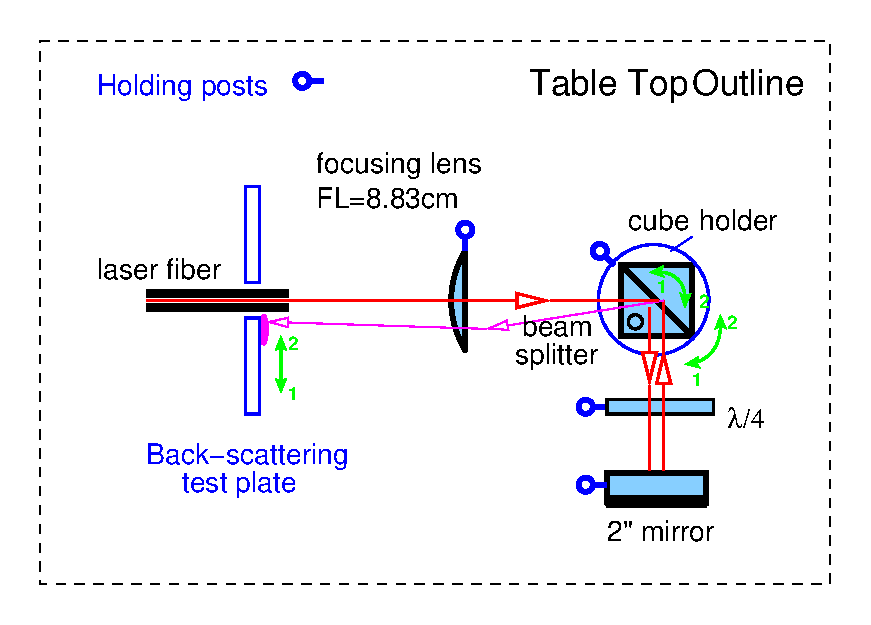
\includegraphics[scale=0.8, angle=0]{laser_detail}}
\end{center}
\caption{Adjusting back-scattering light}
\label{fig:laser_detail}
\end{figure}

\end{itemize}


%-----------------------
\subsection{Operation I: Local Mode}
To turn a laser on:
\begin{enumerate} \setlength{\parskip}{0ex}
\item Be sure to connect the laser control box to the interlock and to
the correct laser.
\item Turn on the switch on the back panel of the laser.
\item Turn the key on the front panel to turn on the power.
\item Set the current through the keypad.
\item Press the On/Off button.  The screen should show 'laser enabled'.
\item Press the On/Off button again.  The screen should show 'laser on'. The 
      laser should be on now.
\end{enumerate}
To turn a laser off:
\begin{itemize}
\item Press the On/Off button.  The screen should show 'laser disabled'.
\end{itemize}

Table \ref{tab:laserparam} lists the optimum parameter
determined for the 30\,W lasers used in early experiments.

\begin{table}[hbp]
\begin{center}
\begin{tabular}{|c|c|c|c|c|c|}\hline

 Laser        & PS \#  &  FAP-I \#  &  Set Current & Set Temperature & Maximum Current $\star$\\ \hline
 Coherent 1   & 3115   &  V7645     & 38500 mA  &   15 $^\circ$C     &  45000 mA\\ \hline
 Coherent 2   & 4151   &  V7250     & 37000 mA  &   24 $^\circ$C     & 44600 mA    \\ \hline
 Coherent 3   & 4157   &  V7251     & 40000 mA  &   26.3 $^\circ$C   & 48000 mA    \\ \hline
 Coherent 4   & 4206   &  V8491     & 40000 mA  &   15.5 $^\circ$C   & 48000 mA    \\ \hline
 Coherent 5   & 4209   &  V8511     & 36000 mA  &   19.7 $^\circ$C   & 43200 mA    \\ \hline
 Coherent 6   & 4208   &  V8492     & 40000 mA  &   14.7 $^\circ$C   & 48000 mA    \\ \hline
 Coherent 7  && & &  &       \\ \hline
 Coherent 8  && & &  &       \\ \hline
 Coherent 9  && & &  &       \\ \hline
 Coherent 10  && & &  &       \\ \hline
\end{tabular}
 $\star$ Factory set absolute maximum current 
\end{center}
\caption{Operational parameters for the 30\,W lasers.}
\label{tab:laserparam}
\end{table}



%-----------------------
\subsection{Operation II: Remote Mode}

For the remote mode to work, 
the lasers must be connected to the interlock box,
the interlock system must be engaged and
the laser key turned on as described above. The lasers can then 
be controlled through the MEDM GUIs:

To turn a laser on:
\begin{enumerate} \setlength{\parskip}{0ex}
\item Set the desired temperature and current in the ``Set Temp'' 
and ``Set Current'' enter boxes.
\item Press the ``Enable'' button.  If you have a camera pointing
at the laser box in the Hall then you should see 'laser enabled'.
\item Press the ``Start'' button.  If you have a camera pointing
at the laser box in the Hall then you should see 'laser on'.  The
laser should now be on.
\end{enumerate}
To turn a laser off:
\begin{itemize}
\item Press the ``Stop'' button.  If you have a camera pointing
at the laser box in the Hall then you should see 'laser disabled'.
\end{itemize}

In addition to cameras pointing at the lasers boxes in the Laser Hut to 
monitor lasers on or off, there is a spectral-analyzer which monitors
both the relative power and the waveform of the lasers. The spectral-analyzer 
has remote readback.  Alarm will be set when the readback deviate
from the regular running condition by more than $10\%$. This will enable us 
to know when there is one laser goes off or when the cell ruptured.

%-----------------------------------------------------------
%\subsection{Quarter-Wave Plate Motion Control}
} % infolev
\infolevone{
%==================================
%\chapter
\section{Target Cell}
\subsection{Description}

The target cell is usually a 40 cm long aluminosilicate glass (GE180)
 high pressure (about 10 atm) double chamber cell. Typical
dimensions for a 40 cm cell are shown in Fig. \ref{fig:cell1}. 
It is a closed system filled with a gas mixture which consists of $^3$He, rubidium and
nitrogen. 

The cell volumes is about 200 ml for a 40 cm cell.
The interior pressure of the cell at room temperature is between 7 and 10 
times atmospheric pressure.  The cells contain approximately 70 torr of 
nitrogen to help with the spin-exchange process.  There is usually 0.1-0.3 g 
of Rb-K mixture with a mixing ratio of 1:5 in the pumping chamber.  
The tritium contamination of the $^3$He gas 
used to fill the cell is less than 10$^{-11} \%$ according to 
the specifications from the manufacturer, Spectra Gases.

The glass walls of the cell vary in thickness from cell to cell 
and from chamber to chamber.   The end windows of the target chamber 
are 120-150 microns thick and are therefore the thinnest part of the cell.  
The walls of the target chamber and transfer tube are over a millimeter 
thick and the pumping chamber walls are up to 2 mm thick.   

\begin{figure}[t]
\begin{center}
\centerline{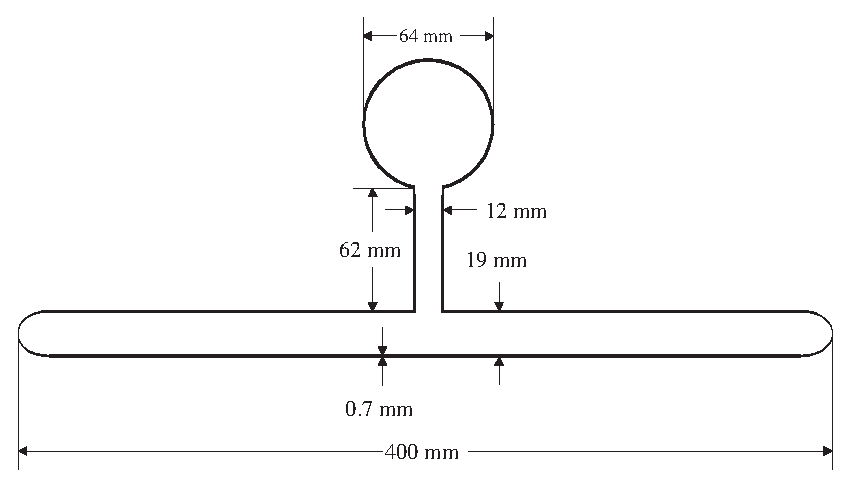
\includegraphics[scale=1]{tcell}}
\end{center}
\caption[Typical 40 cm polarized $^3$He target cell]%
{Typical 40 cm polarized $^3$He target cell used in this
experiment.}
\label{fig:cell1}
\end{figure}

The cell is installed on a target ladder and then this ladder is
mounted to the bottom of the oven.  The cell is attached to the target
ladder with a high-temperature elastomer, GE RTV106.  The ladder is
then bolted onto the oven.


\subsection{Installation \& Replacement}

\begin{safetyen}{10}{5}
The target installation is a delicate procedure and should be
performed only by qualified personnel. A minimum requirement is
Radiation Worker II training.  Only the first time installation does
not require the monitoring of radiation around the pivot area. After
the cell has been exposed to the electron beam, any replacement of the
cell must be done under strict observation of possible radiation and
contamination hazards.

The cells are fragile and under high pressure so they can cause damage
not only to exposed skin and eyes, but also hearing.  It is therefore
important to wear hearing protection in the vicinity of an exposed
cell and also to wear a face shield and a safety glasses when handling
or in the vicinity of someone handling a cell.

\end{safetyen}

In the following we describe the procedure for cell replacement. The
procedure applies both to a routine replacement and a replacement
after a cell  explosion.

\begin{itemize}
\item 
If the replacement of the cell follows the explosion of a previous
target, a new $Q$ curve of the pickup coils should be measured. If the
pickup coils have deteriorated, they should be replaced as well.

\item
Lasers should all be tunne off. Laser fibers be disconnected from the lasers
and be lock-away following the lock-and-tag procedure.

\item 
Prepare the replacement target and, if necessary, a new set of
pickup coils. Request Hall access from MCC, and wait for a member from
the RADCON team to accompany the group of qualified people authorized
to change a target cell.

\item  
The member of the RADCON group will evaluate the radiation level
around the target area. If safe levels of radiations are observed, the
work can proceed. Otherwise a Radiation Work Permit will have to be
written. The member of the RADCON group will either clean up the 
glass pieces or, after determining that there is no contamination, informs 
us that we can proceed to clean up the glass pieces.

\item 
\begin{safetyen}{10}{5}
All personnel within the target area platform must wear ear
protection, a face shield and a pair of safety glasses 
during any access to the inside of the target enclosure.
\end{safetyen}
\item  
Remove the side enclosure to provide sufficient
access to the target.  
\begin{safetyen}{10}{5}
Monitor the radiation level close to the target
ladder and oven.  Determine what conditions are required to comply
with a radiation safe work condition.
\end{safetyen}

\item 
Qualified personnel should proceed to replace the target and align it
according to well defined reference lines of the target ladder. The
motion of the target and the clearance between the pickup
coils should be tested. When finished,
the enclosure should be put back in place. 

\item 
\begin{safetyen}{10}{5}
If an intact target cell was removed, it should be stored in a wooden
box with a screwed lid or a metal box specially designed for store
target cell. It must be left in the hall with 
``Pressurized Glass Cell, Open By Authorized Personnel Only'' warning sign 
on the box. It can only be
removed from the Hall after approval from RADCON.
\end{safetyen}

\end{itemize}

} % infolev
\infolevtwo{
%-----------------------------
%\chapter
\section{Target Ladder \& Motion System}
\label{sec:motion}

\subsection{Description}


        The polarized $^3$He target system has five target positions:
the actual polarized target cell, which can be replaced by a water
cell for NMR calibration (see Section \ref{sec:nmr}), a solid
BeO target inline with a seven-foil Carbon target for alignment and
optics calibration, a ``hole'' target for alignment,
an empty target position that contains no target
and allows the beam to pass undisturbed through the apparatus, and
a reference cell position (see Section \ref{sec:refcell}).
These targets are mounted on a target ladder as shown in Fig.
\ref{fig:tgtladder}.

\begin{figure}
\begin{center}
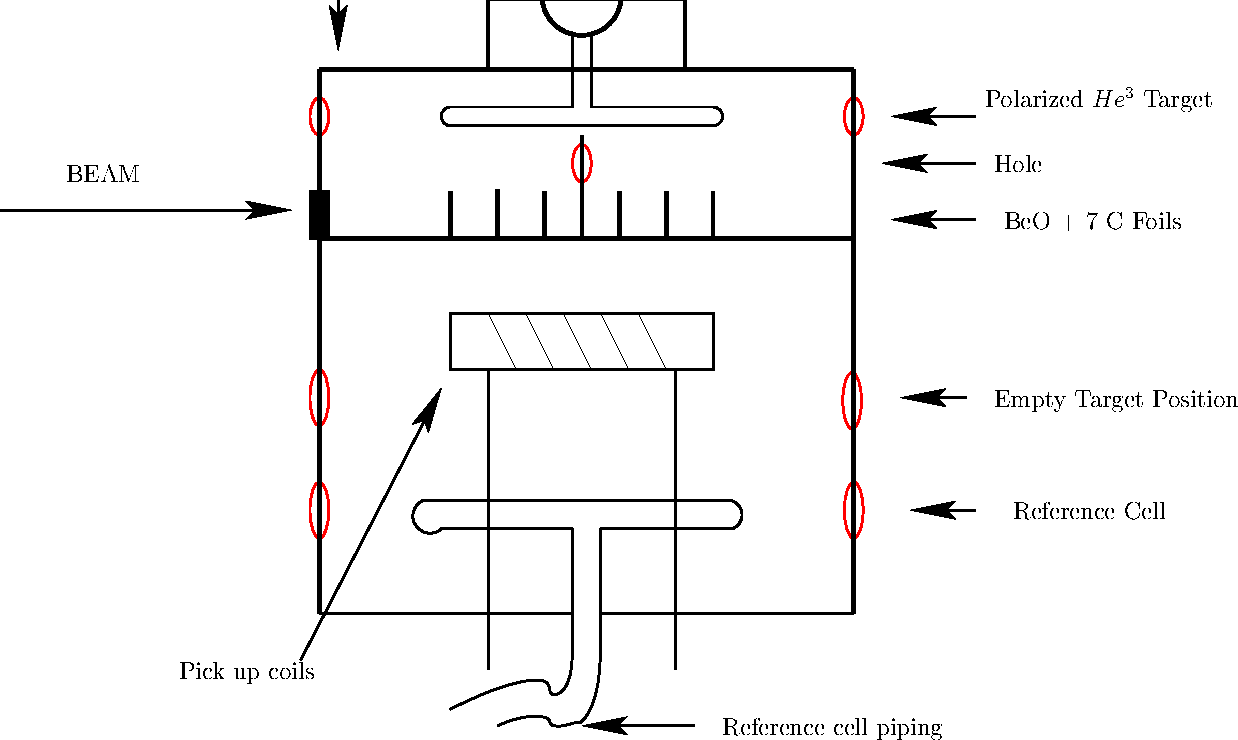
\includegraphics{targetladder}
\caption{Schematic diagram of the target ladder and target positions.}
\label{fig:tgtladder}
\end{center}
\end{figure}

        The target ladder can be positioned vertically using a  
stepper-motor-driven motion control system.  The controller can drive the
ladder to six different fixed positions, four of which correspond to
the four targets, the fifth to the empty (no target) configuration,
and the sixth to the position used for NMR measurements where the
target cell is surrounded by the pick-up coils.  
%The total required vertical motion range is approximately 15\,cm.

        The motion controller employed was developed at JLab and has been 
used for previous experiments.
Vertical target motion is provided by a screw-driven cylinder 
(Industrial Devices Corporation model N2P22V1205A12MF1MT1L).  
The cylinder incorporates a 200 step/rev 
stepper motor with a 1:12 gear, resulting in a position repeatability 
of about $\pm 13 \,\mu$m at a maximum load of 600 lbs (272\,kg). 
The maximum range of motion is 31.5\,cm.  Mechanical position 
sensors are mounted on the target support frame to indicate motion
limits.  These switches are wired normally closed and fail
open.  A magnetic position sensor (Reed Sensor, PSR-1Q) mounted 
on the motor cylinder serves as the home switch.  This switch is
wired normally open, using only two of its three wires (12 V is not 
connected for this type of switch).  Additionally, a linear 
potentiometer provides independent readback of the cylinder position.

\subsection{Operation}
        The motor can be controlled locally and remotely.  Local control
is provided through the SmartStep 23 keypad controller.  The keypad 
allows the target to be jogged into position.  It also allows for small
codes to be saved which will move the target ladder into preset target
positions.  Remote control is provided through the EPICS environment.
During norml operation, target motion is controlled through the lifter
MEDM GUI running on one of the computers in the Hall A counting house.
The GUI has
buttons for preset target positions, as well as lights
indicating the status of the controller (i.e. any faults, at a limit, etc.).
The velocity, acceleration time, deceleration time and position can
also be manually set from the GUI, but the defaults should be correct
for all but special situations.  The position of the motor is readback
on the GUI.  This position is displayed in revolutions from the home
position and can be compared with preset target positions.  

        The electronics provide a Fast Shutdown (FSD) interlock signal 
to the accelerator that is triggered whenever the target is moved with
the beam on.  This prevents damage to the target
cell and ladder due to the electron beam.  The FSD signal is generated
by the SmartStep controller and sent to an FSD node in the Hall.
Target changes require Hall A personnel to telephone MCC and request
temporary masking of this FSD channel.
} % infolev
\infolevone{
%-----------------------------
%\chapter
\section{Target Enclosure \& Windows}

The target is surrounded by an enclosure similar to a scattering chamber.
The enclosure serves three purposes: First, it is part of the laser light 
enclosure. Second, it provides a
containment volume in case of explosion of the target cell and so limits
the potential hazard working area. 
Third, it allows the region around the target to be filled
with helium gas, minimizing ionization and energy loss of the electron 
beam crossing the target area.

The enclosure is made of HDPV material and the middle section is removable
for access to work in the target area.

\begin{safetyen}{10}{5}
If the middle section is open, people working anywhere on the {\em target
platform} must wear ear protection and a face shield. Lasers should have been
tuned off and fibers be locked away following the lock-and-tag procedure.
This region is
designated as the ``target area''.  Signs will be posted indicating
that the enclosure is open and that work is in progress. If the enclosure
is closed the target area is no longer restricted except for possible
reasons of radiation safety.
\end{safetyen}

The electron beam line is under vacuum and separate from
the target enclosure for both upstream and down-stream of the target
enclosure with the enclosure windows.  The beam inlet and
outlet windows of the target enclosure are made of 0.127mm and 0.254mm) 
thick Be and are strong enough to stop any flying glass shreds in case
of a target cell explosion.
} % infolev
%-----------------------------
\infolevone{
%===================================
%\chapter
\section{Target Cell Heater}
\label{sec:tgtheater}

The target pumping cell must be kept at a temperature of about
230$^\circ$C for optical pumping of Rb-K to be
effective. This is accomplished by flowing hot air through a special
temperature-resistant enclosure (``oven'') around the pumping cell 
and regulating the temperature of the air using a process
controller. The system is described in detail in the following.

%----------------------------------
\subsection{Description}
Fig. \ref{fig:oven} shows a schematic diagram of the heater system
and the associated controls. Pressurized dry and filtered air at room 
temperature is provided by a dedicated compressor in the Hall. The air
enters the system through a shut-off valve and a pressure regulator,
which is typically set to an output pressure of 15 psi. The flow rate
is measured with a gas velocity sensor (Omega model FMA-905) connected
to a display unit (Omega DP41-E-S2R) that provides an alarm
to indicate insufficient flow. The air then passes through two
resistive heaters (120 VAC, 1200 W)\ and continues through
insulated copper tubing into the target oven. The
oven material is ceramic which can withstand a
temperature of at least 300$^\circ$C continuously.
The air finally exits the system through an exhaust pipe 
where it can cool down. Both inlet and exhaust pipes are inside the oven 
supporting tube filled with insulation material.

\begin{figure}
\begin{center}
\centerline{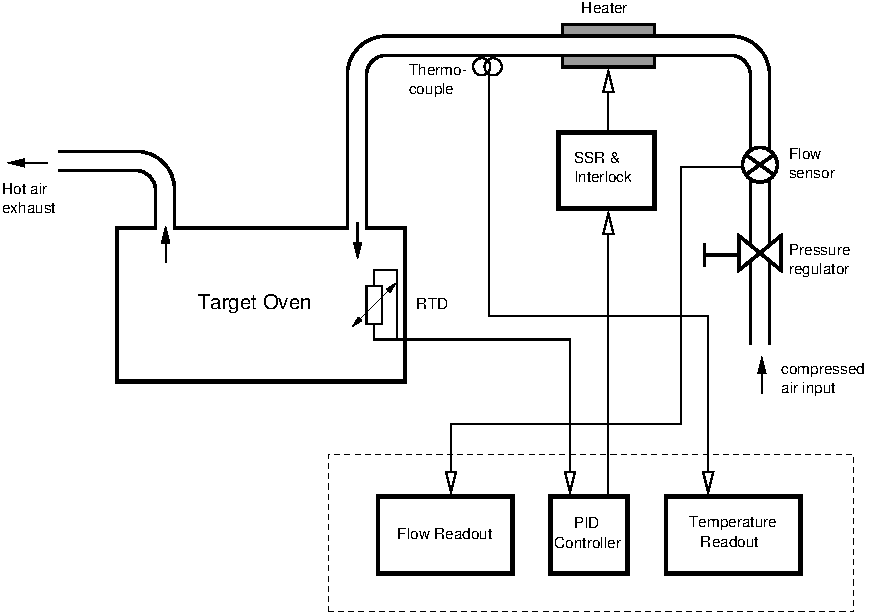
\includegraphics{ovensystem}}
\end{center}
\caption[Schematic diagram of the target cell oven control system]%
{Schematic diagram of the target cell oven control system. The
instruments in the dashed box are located upstairs, while the remaining
components are located in the Hall in the vicinity of the target. 
For clarity, the interlock circuitry
is not shown (see Fig. \protect\ref{fig:interlock}).}
\label{fig:oven}
\end{figure}

\begin{figure}
\begin{center}
\centerline{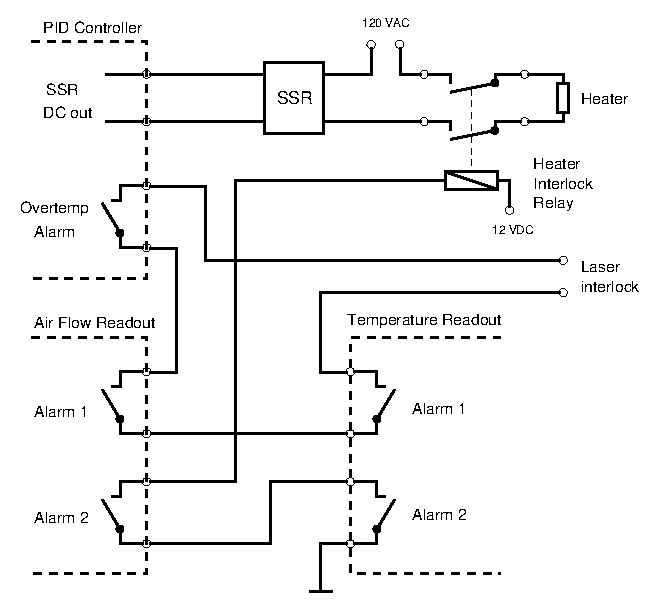
\includegraphics{interlock}}
\end{center}
\caption[Schematic diagram of the oven heater interlock system]%
{Schematic diagram of the oven heater interlock system.
The switches represent relays. 
In normal operation, the relays are energized (contacts closed). 
An alarm condition
(or instrument power failure) will de-energize (open)
 the corresponding relays,  interrupting the interlock circuit.
The instruments are programmed such that their dual alarm outputs
operate simultaneously.}
\label{fig:interlock}
\end{figure}


A 100$\Omega$ Pt RTD (Omega model F3105) measures the temperature
inside the oven. A process
controller (Omega CN77540-C2) operating in PID mode drives the
heater via a solid-state relay (SSR) regulating the heater power
dependent on the temperature detected by the RTD.
The SSR (Omega model SSR240DC10) accepts a low-voltage (3 $-$ 32 VDC)
control signal of about 30 mA. A mechanical relay between the SSR and
the heater allows interruption of the 120 VAC heater power in case of a 
malfunction (see subsection \ref{sec:heaterinterlock}).

A thermocouple (Omega 5SC-GG-K-30-36) is mounted on the
tubing right after the heater to allow monitoring of the temperature
of the air exiting the heater.  Another display unit (Omega
DP41-TC-S2R) reads the thermocouple and generates an alarm if the
temperature exceeds a preset threshold.

The PID controller as well as the two display units are installed
in a 19'' chassis in the electronics racks on the second floor of the
counting house where they can be manually operated if necessary.
All other components are located in the Hall in the vicinity of the
target. The instruments can be monitored
and programmed remotely via serial RS-232 communications, which
allows convenient control via an EPICS/MEDM graphical user interface 
(GUI) in the counting house.

\begin{safetyen}{10}{5}
\subsection{Safety Considerations}
\label{sec:heaterinterlock}

The heater system represents a significant fire hazard and therefore
requires good failsafe protection.
Possible failure modes include:
\begin{enumerate}

\item Insufficient air flow. Possible causes: Compressor failure;
obstruction
  in filter; operator error. Possible harzards: Overheating of heater
element,
  resulting in equipment damage and/or fire.
  Protection: Air flow is monitored; insufficient flow disables heater
  (and laser) via hardware interlock.
\item Heater overtemperature. Possible causes: Insufficient airflow;
  temperature controller failure; RTD failure; operator error.
  Possible hazards: Damage to heater element and/or tubing; fire.
  Protection: Heater temperature is monitored; excessive temperature
  disables heater (and laser) via hardware interlock.
\item Oven overtemperature. Possible causes: Temperature controller
failure;
  RTD failure; insufficient air flow; excessive laser power; 
  operator error. Possible hazards: Explosion of target cell; damage
  to oven enclosure and/or optical elements; fire.
  Protection: Temperature controller will generate alarm if RTD
indicates
  excessive temperature, disabling heater via internal logic and 
  and laser via hardware interlock. 
%  Auxiliary RTDs inside oven are continously monitored by EPICS control 
%  program; excessive temperature disables oven controller via software.
\end{enumerate}

A schematic diagram of 
the interlock system is shown in Fig. \ref{fig:interlock}.
The instruments are programmed such that their dual alarm relays
operate simultaneously if a value is out of range.
An interlock condition disables the heater as well as puts the
lasers in standby mode. Interlocking the
lasers is important as the laser light contributes significantly to
the heating of the target oven. 

\end{safetyen}

\subsection{Operation}
The oven can be controlled from a GUI running
on one of the Hall A counting house computers, or manually using the
front panel controls. 

\subsubsection{Local Operation}
A brief description of the manual operating procedure is given here:

\begin{enumerate}
\item The oven controller and temperature and flow displays are located
  in a 19'' chassis in one of the racks upstairs. Make sure power to this
  chassis is on. The green light on the front panel should be lit.

\item Verify the alarm set points for the flow meter and
  temperature indicator. Press the {\tt SETPTS} button
  until the display shows {\tt SP3}. After about 1 second,
  the setpoint value appears. It should be 250 for the
  air flow display and 220 for the temperature display. Press
  {\tt SETPTS} again and check setpoint {\tt SP4}. It
  should be identical to {\tt SP3}.

  To change
  any of the values use the {\tt MIN} and {\tt MAX} buttons. The {\tt MIN}
  button selects the digit to be changed whereas the {\tt MAX}
  button changes the value of the currently selected digit.
  Press {\tt SETPTS} again to store the new value. 
  When finished, press {\tt SETPTS} until {\tt RUN} appears in the
  display.


\item Verify the current temperature of the oven. It is shown
  in the upper (red) display of the temperature controller
  and is labeled {\tt PV} for ``Process Value''. The units are $^\circ$C.
  The value should be reasonable,
  {\it e.g.}\/ around room temperature if the oven has been off
  for several hours or more. If the value does not make sense,
  either the controller is misconfigured (see below) or the RTD 
  in the oven is broken or incorrectly connected. 
  Do not proceed before you have a sensible reading.

\item (Optional) Verify the correct configuration of the controller.
  Use the {\tt MENU} button on the controller to scroll through
  the various configuration menus. To inspect parameters within
  a menu, press {\tt ENTER} followed by {\tt MENU} again. The suggested
  default parameters are listed in Tables \ref{tab:ctlparam1}
  and \ref{tab:ctlparam2}. This step
  is time-consuming and can be skipped if you are relatively certain
  that the configuration is ok. A detailed description of the 
  controller parameters is given in the controller manual.

\item Verify that air is flowing. The air flow readout should indicate
  a value of 350--450. These are arbitrary units. As long as the heater is
  off, the reading should not fluctuate by more than about $\pm 10$ units.

\item Verify the current temperature of the heater. It should be
  close to room temperature. If the value is unreasonable, either
  the readout is misconfigured or the thermocouple is broken.
  Do not proceed before the problem is corrected.

\item Verify that alarms are reset. 
  Underneath the main display there are four LEDs, one for each
  alarm 1--4. If either LED {\tt 3} or {\tt 4} is on on either
  instrument, it indicates that an alarm has been triggered and
  that the system is interlocked. You must reset the alarms before
  you can continue. To do so, first correct
  the problem ({\it e.g.}\/ turn the air flow on) then press {\tt RESET}
  once on the affected instrument(s). If the LEDs stay on despite
  correct setpoints and readings, the instrument is probably misconfigured.

\item Begin heating. 
  To avoid damage to the oven, the temperature must be increased
  to the final value slowly. A good final operating temperature is
  170$^\circ$C, and a good ramping rate is 60$^\circ$C/h, {\it i.e.\/}\
  heating of the oven will take about three hours to complete.
  
  In manual mode, you must enter a new temperature setpoint by hand
  at fixed time intervals. (``Ramp and Soak'' does not seem to work reliably
  with this controller.) You should increase the  value by
  10$^\circ$C every 10 minutes. For example, if the current oven temperature
  is 35$^\circ$C, start with a setpoint of 45$^\circ$C and increase this
  value by 10$^\circ$C in approximately 10 minute intervals.

  To enter a new setpoint, do the following
  \begin{enumerate}
   \item Press {\tt MENU} on the temperature controller. 
         A little green light marked {\tt SP1} in the upper left corner of 
         the display will start to blink. Also, the first digit of
         the green numerical display, labeled {\tt SV} for ``Setpoint
         Value'', will blink.
   \item Use {\tt MIN} to select the digit you wish to change and {\tt MAX}
         to modify the value.
   \item When done, press {\tt ENTER}. The display will briefly show
         {\tt run} when the controller enters normal operating mode.
         This starts the heating process.
  \end{enumerate}

\item Check correct operation of the controller. A little green 
  light marked {\tt SP1} in the upper left corner of the 
  temperature controller display indicates that the heater is active.
  This light should blink slowly, being mostly on while the oven is heating
  up and being mostly off (or even completely off for periods of up
  to a few minutes) when the oven temperature has reached the setpoint.

  The heater temperature should increase proportionally to the
  fraction of time that the {\tt SP1} indicator is on. 
  Note that the temperature reading is {\it not} directly related to the
  oven temperature. In particular, the heater may become significantly
  hotter than the oven, and its temperature 
  might fluctuate from almost room temperature
  to high values over short periods of time as the heater 
  power is automatically
  cycled on and off by the controller.  As long as the temperature 
  stays below the alarm threshold (220$^\circ$C) there is no reason 
  for concern.

\item Check stability of the final temperature. 
  The temperature might overshoot slightly. If the overshoot is
  less than about 5$^\circ$C then this is normal. If the stability is
  poor it is probably due to incorrectly set PID parameters in the controller. 
  Changing these parameters is best done by an expert since this requires
  in-depth understanding of the system.

  The laser contributes significantly to the heating of the oven.
  Therefore, you will notice sudden temperature instabilities when
  the laser is turned off or on. It will take several minutes for
  the controller to compensate for such changes.

\item The air flow rate is slightly dependent on the heater power
  applied (conductance varies with temperature). 
  Therefore, the flow rate will fluctuate by some 10-20\%. This is
  normal.


\item At any time you can place the controller in standby mode by pressing
  {\tt ENTER} twice. The display will show a blinking text {\tt STBY}.
  This will turn the heater off completely and can be used
  when the system appears to malfunction.   However, exercise some
  caution if the oven is at an elevated temperature since it will quickly 
  cool down if heater power is disabled and you will lose time bringing
  it back up to operating temperature.

\item In an emergency, simply turn the power to the chassis off completely.
  This will open the interlock loops, thereby cutting power to the heater
  and placing the laser in standby mode.

\end{enumerate}

\begin{table}
\begin{center}
\begin{tabular}{|l|l|r|}
\hline\hline
Menu & Submenu & Setting \\
\hline
Output Redirection  &                        & S1.o1 \\
\hline
Input Type          &                        & RTD   \\
                    & RTD Type               & 385.3 \\
                    & RTD Value              & 100\_  \\
\hline
RDG Configuration   & Decimal Point          & FFF.F \\
                    & Temperature Units      & $^\circ$C \\
                    & Filter Constant        & 0004 \\
\hline
Alarm 1             &                        & Enabled \\
                    & Type                   & Absolute \\
                    & Latched                & Latched \\
                    & Contact                & n.c. \\
                    & Setup                  & Above \\
                    & Power On               & Enabled \\
                    & Low Value              & (anything) \\
                    & Hi Value               & 210.0 \\
\hline
Alarm 2             &                        & Not Installed \\
\hline
%%% xxx should enable later!
Loop Break          &                        & Disabled \\  
\hline
Output 1            & Self                   & Disabled \\
                    & \% Low                 & 0000 \\
                    & \% High                & 0095 \\
                    & Control Type           & PID \\
                    & Action Type            & Reverse \\
                    & Auto PID               & Disabled \\
                    & Adaptive Control       & Disabled \\
                    & Anti Integral          & Enabled  \\
                    & Start PID              & Disabled \\
                    & Proportional Band      & 0038 \\
                    & Reset Setup            & 0050 \\
                    & Rate Setup             & 0000 \\
                    & Cycle Time             & 0001 \\
                    & Damping Factor         & 0001 \\
\hline
Output 2            & (any)                  & (anything) \\
\hline
\end{tabular}
\end{center}
\caption{Suggested default parameters for the temperature controller.}
\label{tab:ctlparam1}
\end{table}
%-----------------------------
\begin{table}
\begin{center}
\begin{tabular}{|l|l|r|}
\hline
Menu & Submenu & Setting \\
\hline
Ramp \& Soak        & Ramp                   & Disabled \\
                    & Soak                   & Disabled \\
\hline
Analog Output         &                      & Not installed \\
\hline
Communication Option  & Baud                 & 9600 \\
                      & Parity               & Odd  \\
                      & Data Bits            & 7bit \\
                      & Stop Bits            & 1bit \\
\hline
Bus Format            & Checksum             & no  \\
                      & Line Feed            & no   \\
                      & Echo                 & no   \\
                      & Standard             & 232C \\
                      & Mode                 & Command \\
                      & Separator            & Space   \\
\hline
Data Format           & Status               & yes     \\
                      & Reading              & yes     \\
                      & Peak                 & no      \\
                      & Valley               & no      \\
                      & Unit                 & yes     \\
                      & ID                   & no      \\
\hline
Address Setup         & (any)                & (anything) \\
\hline
Transmit Time         & (any)                & (anything) \\
\hline
Remote Setpoint       &                      & Not installed \\
\hline\hline
\end{tabular}
\end{center}
\caption{Suggested default parameters for the temperature controller 
(continued).}
\label{tab:ctlparam2}
\end{table}

\subsubsection{Remote Operation}
\begin{enumerate}
\item Make sure the power is on to the Oven Heater Controller
Chassis as described above.  Also verify the alarm set points
for the oven air flow and heater temperature as above.  
\item Verify the current temperature of the oven.  It is shown
on the GUI on the blue HacOMEGA\_RTD readback.  It's shown on 
the meter and also in the readback box.  Also, a plot of oven temperature
vs time is shown on the stripchart in the bottom-left of the GUI 
(labelled oven temperature).  The units are $^\circ$C. 
The value should be reasonable,  {\it e.g.}\/ around room temperature 
if the oven has been off for several hours or more. If the value 
does not make sense, either the controller is misconfigured (see 
directions for manual control above) or the RTD in the oven is 
broken or incorrectly connected.  Do not proceed before you have 
a sensible reading.
\item Verify that air is flowing. The air flow readout should indicate
  a value of 350--450. These are arbitrary units. As long as the heater is
  off, the reading should not fluctuate by more than about $\pm 10$ units.
\item Verify the current temperature of the heater. It should be
  close to room temperature. If the value is unreasonable, either
  the readout is misconfigured or the thermocouple is broken.
  Do not proceed before the problem is corrected.
\item Verify that alarms are reset.  The alarms are reset by pressing
the ``Reset'' button in the upper-left of the GUI.  
\item Begin heating.  To avoid damage to the oven, the temperature 
must be increased to the final value slowly. A good final operating 
temperature is 230$^\circ$C, and a good ramping rate is 60$^\circ$C/h, 
{\it i.e.\/} heating of the oven will take about four hours to complete.

In controlling the Oven Temperature from the GUI, you must enter a new
temperature setpoint by hand at fixed time intervals.  Enter the desired
setpoint in the ``SP1'' enter box in the lower right of the GUI.  
You should increase the  value by 10$^\circ$C every 10 minutes. 
For example, if the current oven temperature is 35$^\circ$C, start with 
a setpoint of 45$^\circ$C and increase this
value by 10$^\circ$C in approximately 10 minute intervals.
The heater is controlled in PID (proportional, integral, derivative) mode.
It approaches the setpoint according to the PID parameters defined in
the ``Prop. Band'', ``Reset'' and ``Rate'' boxes in the lower-right
of the GUI.  These values can be changed, but the defaults should be 
fine except for special circumstances.
\item Check stability of the final temperature. 
  The temperature might overshoot slightly. If the overshoot is
  less than about 5$^\circ$C then this is normal. If the stability is
  poor it is probably due to incorrectly set PID parameters on the
  GUI.  Changing these parameters is best done by an expert since this 
  requires in-depth understanding of the system.

  The laser contributes significantly to the heating of the oven.
  Therefore, you will notice sudden temperature instabilities when
  the laser is turned off or on. It will take several minutes for
  the controller to compensate for such changes.

\item The air flow rate is slightly dependent on the heater power
  applied (conductance varies with temperature). 
  Therefore, the flow rate will fluctuate by some 10-20\%. This is
  normal.


\item At any time you can place the controller in standby mode by pressing
the ``Standby'' button in the upper-left of the GUI.  
  This will turn the heater off completely and can be used
  when the system appears to malfunction.   However, exercise some
  caution if the oven is at an elevated temperature since it will quickly 
  cool down if heater power is disabled and you will lose time bringing
  it back up to operating temperature.


\item In an emergency, simply turn the power to the chassis off completely.
  This will open the interlock loops, thereby cutting power to the heater
  and placing the laser in standby mode.

\end{enumerate}
} % infolev
\infolevone{
%=============================
%\chapter
\section{Helmholtz Coils}
\label{sec:helmholtz}

The Helmholtz coils are six large rings of coils that
provide a large constant magnetic field.  Three sets are necessary so
that the magnetic field can point in any direction in the horizontal
plane.  
The larger pair horizontal coils each has an inner diameter of 1.45 m and
consists of 272 turns of coil. The smaller set of coils each has an
inner diameter of 1.27 m and is made of 256 turns of coil. Each pair of the
horizontal coils has a resistance of 3 Ohms. 
The vertical coils each has an inner diameter of 1.83 m and consists of
355 turns of coil. The pair of vertical coils has resistance of 4.4 ohms. 

The normal holding field for the target is 25 Gauss which corresponds
to approximately 7.2 Amps of current and 25 Volts in the horizontal coils 
and 7.4 Amps and 33 Volts
in the vertical coils.  However, when
doing an NMR measurement the field gets as high as 32 Gauss, which
corresponds to 9.2 Amps and 32 Volts in the horizontal coils and 9.5 Amps
and 42 Volts in the vertical coils. The maximum field will not exceed
35 Gauss, which corresponding to 10.0 Amps and 35 Volts for the horizontal coils 
and 10.4 Amps and 46 Volts for the vertical coils.

The horizontal coils are power by two KEPCO BOP 36-12D power supplies.
The maximum range of power supplies is 12 A and 36 V.
The power supplies are
controlled by a DC voltage from two Stanford Research
System DS345 Function Generators.  These are in turn controlled by a
LabView Vi running on a PC.  There is a small glitch in the DS345
function generator : there sometimes will be a short drop in voltage
before going to the correct voltage.  This is a problem when rotating
the field, since it causes sudden magnitude shifts which in turn
destroy a little of the target polarization.  This glitch is
compensated for by a specially designed rotation box to which a
Wavetek 80 function generator is attached.  This function generator
compensates for the small decrease in voltage so that the rotation can
be performed smoothly.

The vertical coils are powered by an Agilent 6675A power supply. The
maximum range of power supply is 18A and 120 V. The operation condition 
for the magnet is typically 25-32 Gauss. The maximum field will not excced 
35 Gauss, which corresponding 10.4 A and max 46 V.
The power supply is controlled by a LabView Vi running on a PC.  

Hazards associated with the operation of the target magnet include exposure 
to voltage and exposure to magnetic field. All Hazards are mitigated by the 
use of the engineering and administrative controls detailed below. 

The power supply is located in an electronics rack. Two insulated cables connect the power supply to the magnet. The voltage hazards are electrical shock or 
burns.The hazards are mitigated by:
\begin{itemize}
\item Engineering control:
 \begin{itemize}
 \item Connectors are covered with insulated material.
 \item Magnet is grounded.
 \item Electronic rack is grounded.
% \item The power supplies are set to have a limit of 48 V.
 \end{itemize}
\item Administrative controls:
 \begin{itemize}
 \item Warning signs in front of the power supply and on the magnet wall.
 \item Voltage to be used is not to exceed 48 V for the Agilent power supply.
 \end{itemize}
\end{itemize}

In addition, there is a hazard associated with magnetic field. The maximum
magnetic field is 35 Gauss inside the magnet. A warning sign will be posted 
around the target area. No person with pace maker will be allowed around the target area.

The following personnel have received the proper training. They are the only ones authorized to operate the power supply and the magnets. Names may be added with authorization from the supervisor of the system (Jian-ping Chen,  x7413).

\begin{namestab}{tab:polhel:personnel-magnet}{Polarized $^3$He target: personnel for working with the coils and power supplies}{%
   Polarized $^3$He target: personnel authorized to operate the power supply 
and
the target magnets}
   \JianPingChen{\em Contact}
   \ChiranjibDutta{}
   \JoeKatich{}
   \YiQiang{}
   \VinceSulkosky{}
   \YiZhang{}
\end{namestab}


Attached to the horizontal Helmholtz coils are two smaller sets of
 coils.  These consist of 20 loops of 16 AWG wire attached to smaller DC
 power supplies.  
% This target occasionally has a problem with a
% phenomena known as masing.  This is a loss of target polarization due
% to coupling of the helium nuclei in their higher energy states (such
% as during an NMR measurement) and a coil of wire (the pick-up coils,
% a Rb ring, or some other source).  Masing can be easily identified
% with EPR, and introducing a small field gradient generally makes it
% disappear.  
They can be used to compensate for field gradient to minimize AFP
polarization loss.
These coils can also be used to introduce a field gradient to reduce 
masing effect.

} % infolev
\infolevone{
%=============================
%\chapter
\section{NMR Polarimetry}
\label{sec:nmr}

This guide explains briefly how to perform safely an NMR AFP sweep on
the polarized $^3$He target. Figure.~\ref{fig:NMR_topview}
shows the target setup and explaining the angle conventions of the
polarized target system. 
%Longitudinal field configuration is named if the holding field is
%pointing along the incident electron momentum direction. 

\begin{figure}
  \begin{center}
    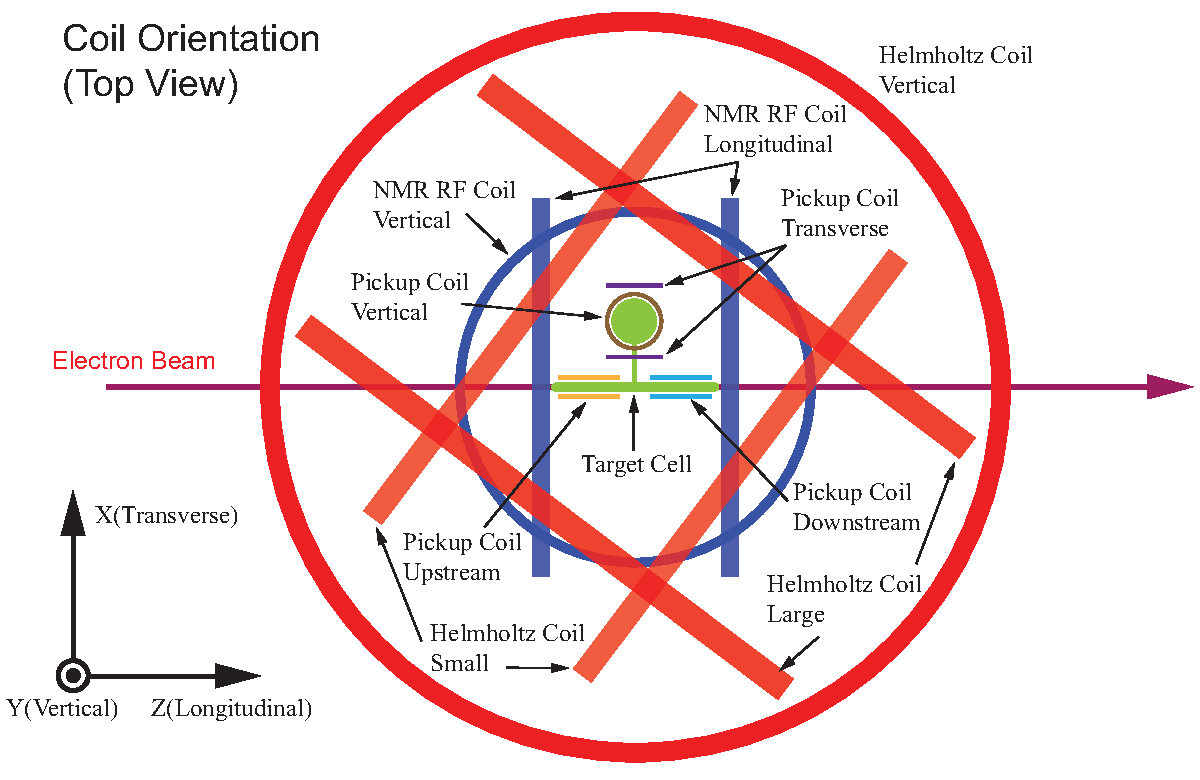
\includegraphics[angle=0,width=.95\textwidth]{coil_setup}
    \caption{Top view of the coils used in the $^3$He target
      setup. The combinations of the 3 pairs of Helmholtz coils power
      the main holding field to either longitudinal, transverse or
      vertical directions while 3 lines of lasers are available as well
      in these three directions to polarize the target.
      The two sets of RF coils are needed to flip the target spin for
      NMR and EPR measurements with different setups field direction.
      Four pairs of NMR pick up coils are used during the flips to
      read out the polarization strength. Two of the pairs are located
      below the beam line to measure the NMR signal from upstream and
      downstream part of the target chamber. The other two of the pairs
      are fixed in the target oven to measure the NMR signal from the
      pumping chamber.}
    \label{fig:NMR_topview}
  \end{center}
\end{figure}

\subsection{NMR polarization measurement}

An automatic NMR measurement will be performed every time when the
target spin gets flipped. Each of these measurement includes:
\begin{itemize}
  \item AFP flip of $^3$He triggered by RF frequency sweep;
  \item Laser polarization change by rotating Q-wave plates;
  \item NMR data recording and automatic polarization calculation;
  \item Spin state determination;
  \item Automatic log entry.
\end{itemize}

For a manual NMR measurement, it has the following steps:
\begin{itemize}
\item Turn OFF the lasers (optional).
\item Make sure the target is in the Helium 3 (beam) position.
\item Make sure the correct RF coil is connected to the
  impedance match box output: use Longitudinal RF coil for
  Transverse or Vertical polarization and use Vertical RF coil for
  Longitudinal polarization.
\item Make sure corresponding impedance is selected in the impedance
  match box.
\item Turn ON the NMR RF amplifier.
\item Make sure the Pumping chamber Lock in amplifier get the signal
  from correct pick up coil: use Vertical pickup coil for Transverse
  polarization and use Transverse pickup coil for Vertical or 
  Longitudinal polarization.
\item Make sure the coil current and oven temperature readings are normal.
\item Call MCC to mask the beam and make sure the target is masked
  before doing anything further. 
  In case NMR signals from target chamber are wanted (only for
  Vertical and Longitudinal polarization), move the target down to the 
  pick-up coils.
\item Run the NMR Measurement VI.
\item Load appropriate parameters by clicking ``Load Default'' button.
\item Start NMR Measurement.
\item Check result and submit log entry by inputing required info.
\item Exit the NMR VI.
\item Move the target back to beam position if previously moved to
  pickup coil position.
\item Call MCC, tell them you have measured the polarization and that 
  the target is back to its beam position. 
  Be sure to follow the beam back procedure before sending the beam
  back to the target (beam position, raster ON and beam current.)
%\item Staple the plots together and store them in the target binder.
\end{itemize}

%\subsection{Plots to print}
%For every NMR measurement, print :
%\begin{itemize}
%\item NMR Record settings panel (will be printed by the Vi)
%\item NMR Measurement panel (print it at the end of the sweep)
%\item NMR Extract Polarization panel (print it when completed)
%\item RTD temperatures screen (print it from the X terminal) 
%  Staple the four plots together and store them in the target binder.
%\end{itemize}

\subsection{Warnings}
\begin{itemize}
\item Never stop a running LabVIEW VI (Normally you can't but don't try
  to hack it);
\item Never put CW beam ON the target without raster;
\item Every target operator must read and sign the Target Operation 
  and Safety Procedure;
\item If the target ruptures, turn OFF the lasers immediately, and
then turn off the heaters;
\item The lasers must be OFF before rotating the holding field;
\item Do not manually change the voltage of the HP6675A;
\item We indicate on Table~\ref{tab:coil_ps} the voltage and current 
  values for each coils power supply.
\end{itemize}

\begin{table}
  \begin{center}
    \begin{tabular}{|c|c|c|c|c|c|}
      \hline
      Coil & Radius (m) & Turns & Power Supply & $I_{Max}$ (A)
      & $V_{Max}$ (V) \\
      \hline
      Small & 0.667 & 256 & KEPCO & 10 & 35 \\
      \hline
      Large & 0.758 & 272 & KEPCO & 10 & 35 \\
      \hline
      Vertical & 0.946 & 203 & HP6675A & 18 & 49 \\
      \hline
    \end{tabular}
    \caption{Maximum condition of the power supplies during $^3$He
      target system operation (35 Gauss).}
    \label{tab:coil_ps}
  \end{center}
\end{table}

\subsection{NMR AFP Safety}
The NMR AFP system provides the DC current in the holding coils (up to
18~A) and the AC current in the RF coils (usually 1~A rms) of the
target setup.
Any human contact with the wires could be fatal and should therefore
be avoided. 
The electronic devices and the PC used to sweep are located in the 
Counting House and Hall A. Refer to Fig.~\ref{fig:ch_layout} and 
Fig.~\ref{fig:NMR_setup} for a description of the electronics.
\begin{figure}
  \begin{center}
    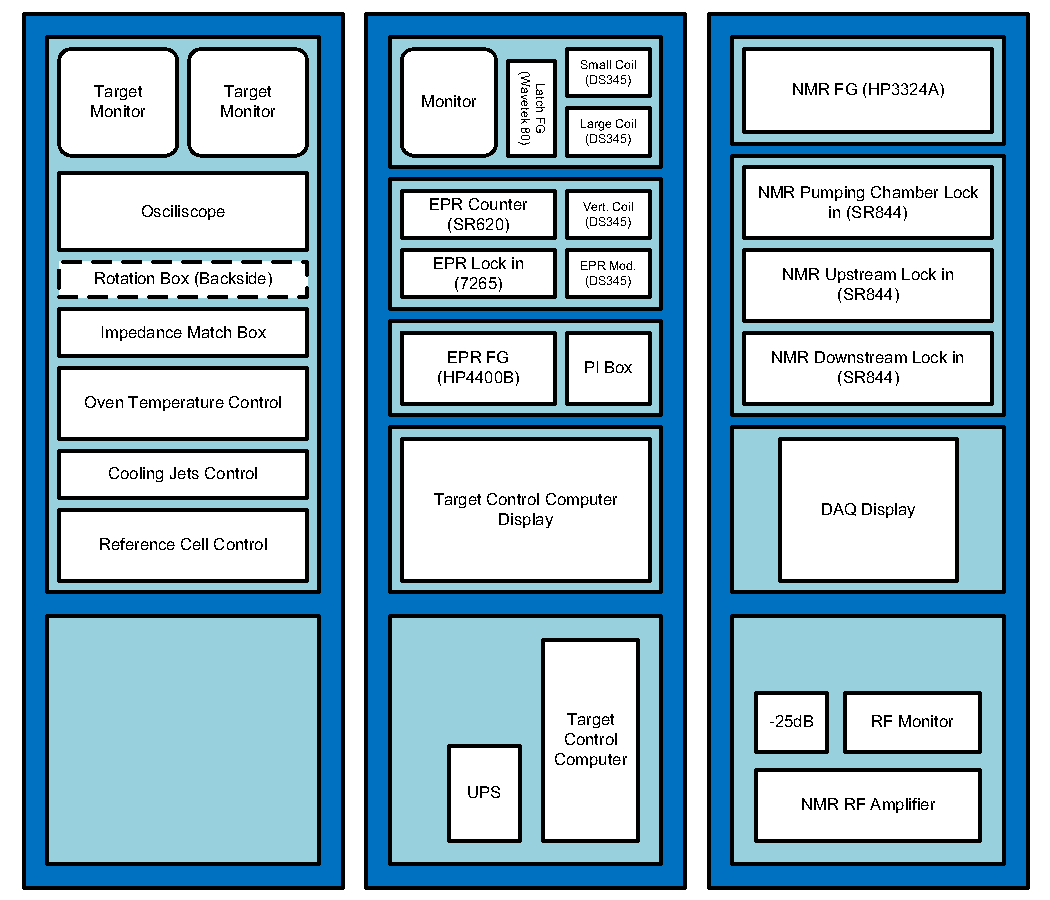
\includegraphics[angle=0,width=.95\textwidth]{ch_layout}
    \caption{The electronics located in the Hall A Counting House.}
    \label{fig:ch_layout}
  \end{center}
\end{figure}

\begin{figure}
  \begin{center}
    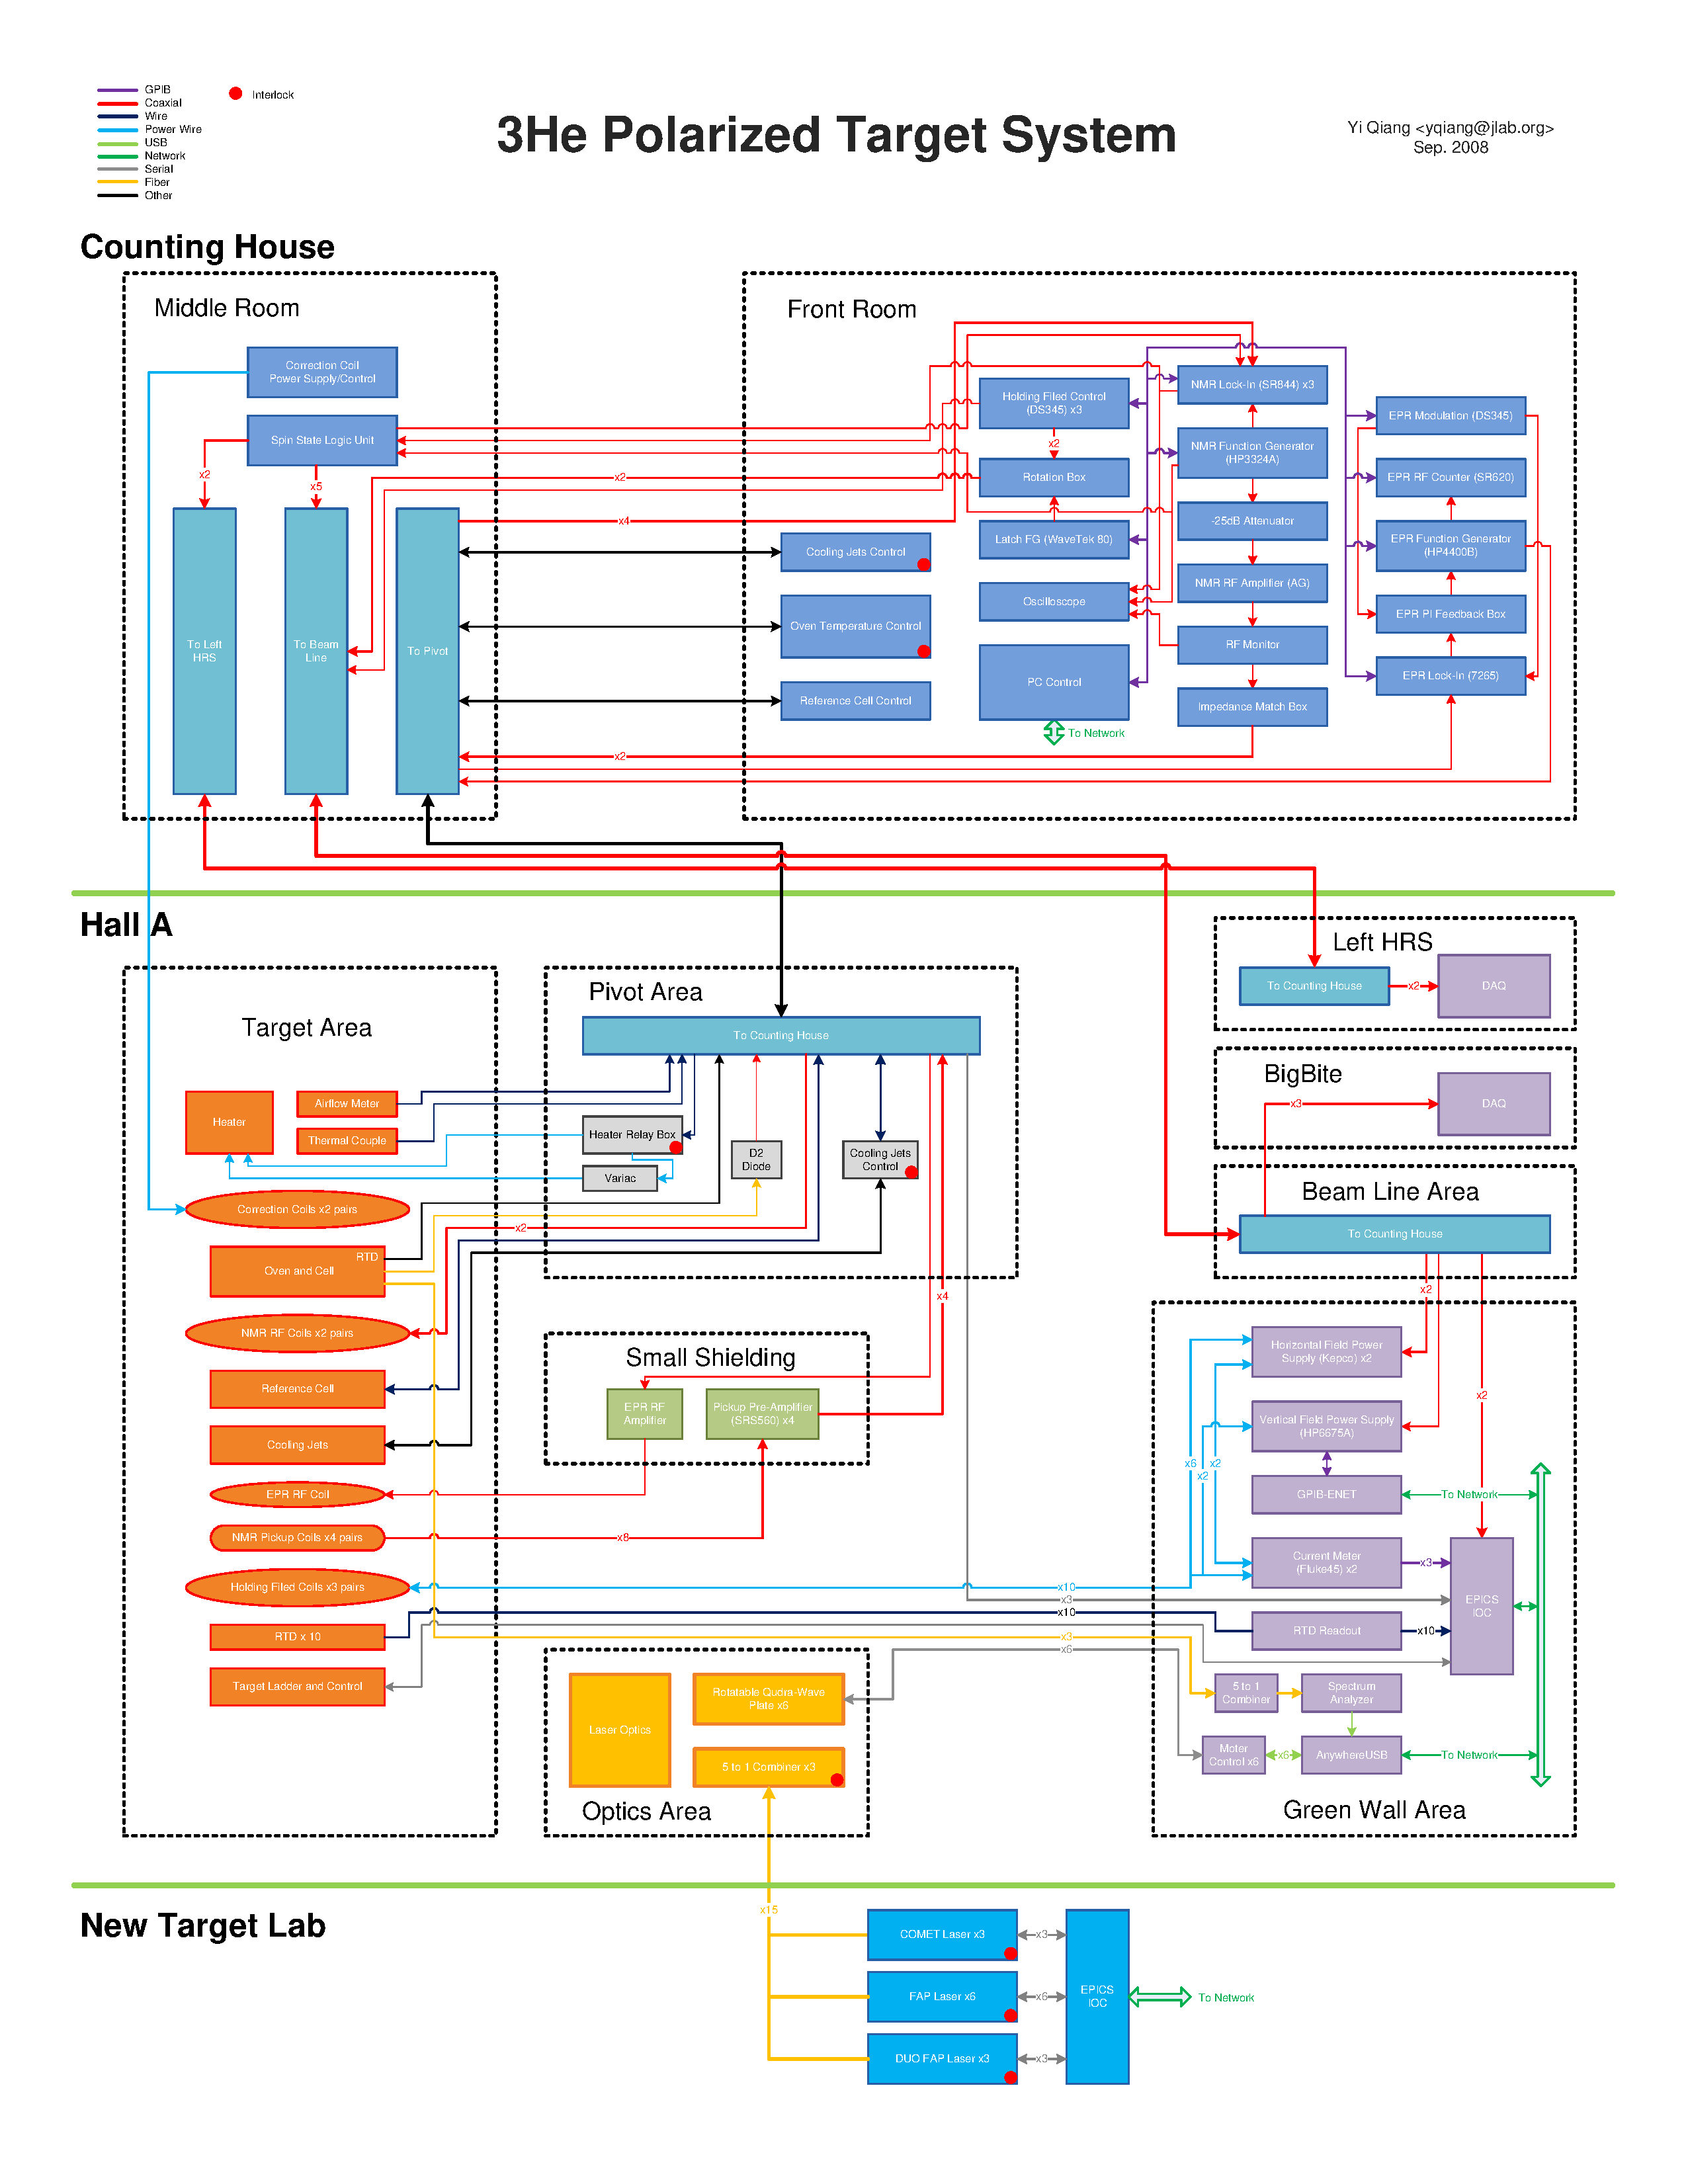
\includegraphics[angle=0,width=.95\textwidth]{Target_System}
    \caption{Complete diagram of Hall A $^3$He target system.}
    \label{fig:NMR_setup}
  \end{center}
\end{figure}

\subsubsection{The DC current}
The DC currents are produced by two KEPCO and one Agilent power
supplies located in a rack behind the green wall in Hall A. 
One KEPCO drives the large horizontal coils, and the other
drives the small ones, as stamped on their front panel.
The Agilent drives the vertical coils. The output of each KEPCO
consists of four wires, two to lead the current, and the two others 
used for sensing. The Agilent has two wires.
The output plugs are located on the back panel of each power supply 
which can only be reached through the back panel of the rack. 
All connections are protected either by plastic strips or covers and 
can not be touched directly by hands.
At the coil end, simple metal screws are used to connect those wires 
to the coils. The connections to the horizontal coils are wrapped by
electric tape and the connections to the vertical coils are shielded
by shrink tubes. They should never be touched while power is ON.
All power supplies are grounded to the ground of the hall.

\subsubsection{How to turn the Power Supplies OFF in an emergency?}
\begin{enumerate}
\item Turn the Function Generators SRS DS345 OFF (one for each coil) 
  by pressing the ON/OFF switch.
\item Turn the KEPCO power supplies OFF by setting the manual ON/OFF 
  switch to the OFF position. The digital displays should turn OFF.
\item Turn the Agilent ON/OFF switch to OFF.
\end{enumerate}

\subsubsection{The AC current}
It is produced by the AG Series Power Amplifier located at the bottom 
of the right rack in counting house. 
When it is running, the power switch is set to the
ON position, the yellow LED is steady and the display shows loaded
power above zero. 
The AC current comes out from the BNC OUTPUT plug, goes through a 
current monitor (looks like a small toroid) and finally goes to the 
RF coils. 
In the hall, the cable is connected to the RF coils along the RF
mounting using simple connectors with screws. 
Those are protected by electrical black tape. 
They should never be touched when the RF Power Amplifier is running. 
The grounding of the system is provided by the RF Power Amplifier.

\subsubsection{How to turn the RF Power Amplifier OFF in an emergency?}
\begin{enumerate}
\item Turn the Function Generator HP 3324A connected to the RF Power 
  Amplifier OFF.
\item Turn the RF Power Amplifier OFF by setting the power ON/OFF 
  switch to the OFF position. 
  All LEDs should turn OFF.
\end{enumerate}

Detailed description of the NMR system is contained in the Hall A wiki
page:
http://hallaweb.jlab.org/wiki
%following technical note by S. Incerti: The NMR system of the Hall A 
%polarized Helium 3 target, JLab-TN-98-049.
%A copy of this note is included in the target binder in the Hall A 
%counting house.

} % infolev

\infolevone{
%======================================
%\chapter
\section{EPR Polarimetry}
\label{sec:epr}

  
In what follows we describe two methods to setup and perform an EPR
measurement of the target polarization.

\subsection{EPR Lineshape Measurement -- Frequency Modulation Sweep:} 
\label{sec:eprfms}

Use this configuration when you wish only to find the Electron
Paramagnetic Resonance (EPR) frequency,
not actually track its position.  This method allows the user to observe
the lineshape of the
EPR transition (Rb D2 line or K lines) light emitted from the cell as a function of applied
frequency to the EPR coil. \\

First, construct the circuit described in Fig. \ref{fig1:epr} by
following these steps:

\begin{figure}
\begin{center}
%\centerline{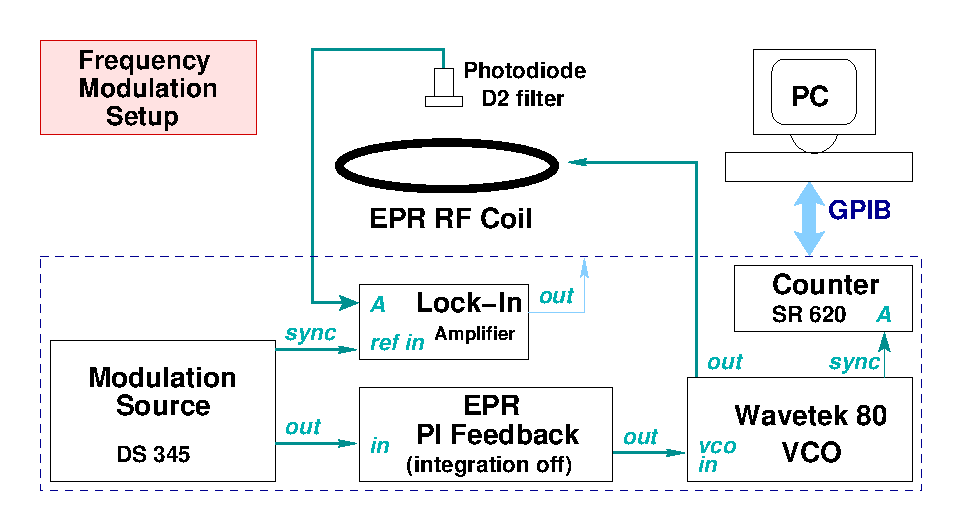
\includegraphics[scale=0.7]{eprfig1}}
\centerline{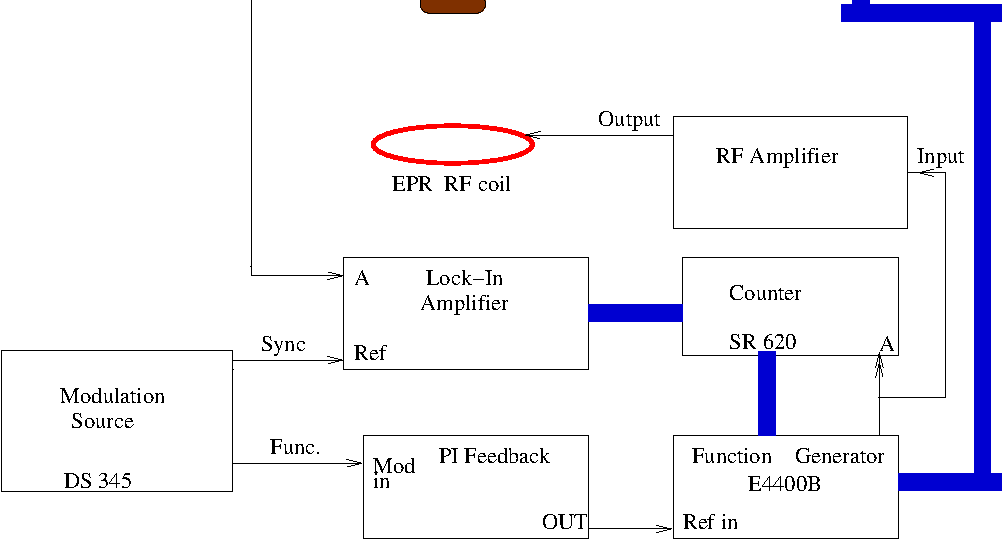
\includegraphics[scale=0.7]{eprfm}}
\caption{Circuit for EPR lineshape measurement}
\end{center}
\label{fig1:epr}
\end{figure}

\begin{enumerate}

\item 
Position the EPR optical fiber so that it looks directly at the light beam
coming from the cell.  Adjust and align the focusing lenses such that 
most of the light is collected through the optical fiber
and reaches the PIN diode.

\item Measure PIN diode output, it should be a DC signal with an amplitude
of -100 mV to -150 mV (could be as high as -230 mV).  
If the signal is less than -100mV, check the light and PIN diode again.

\item Set Lock-in amplifier parameters:\\
\indent    AC Gain:     50 dB;    \hspace{3.2cm}    Input Limit: 10 mV;\\
\indent    Sensitivity:  1 mV;    \hspace{3cm}    DR 16;\\
\indent    Time Constant: 100 ms; \hspace{2cm}    Osc: 0.000 Hz;\\

\item Connect PIN diode to input A of the Lock-in amplifier.

\item Set Modulation source DS345 parameters:\\
\indent     Function:  sine wave;\\
\indent     Sweep/modulate: LIN SWP.\\

\item Connect DS345 'output' to PI circuit 'mod in', 
DS345 'sync output' to Lock-in Amplifier 'ref in'.

\item Set PI circuit Integration off, make sure the input is disconnected.

% The following part is for when Wavetek 80 is used:
%\item Set Wavetek 80 parameters:\\
%\indent Modulation Mode: \hspace{0.5cm} VCO;\\
%\indent Output: \hspace{2.3cm}  sine wave;\\
%\indent Operating mode: \hspace{0.8cm}  FUNC.\\
%
%Be sure that the VCO indicator is lit.
%(The VCO is used because it is very sensitive to small changes in voltage.  
%At a carrier frequency of 10MHz, a 1mV input will produce a 400Hz shift 
%in the output frequency.)
%
%\item Connect PI circuit output to Wavetek 80 VCO IN through an 100:1 
%attenuator. Set the 100:1 attenuator switch to ``FMS'' (no attenuation). 
%
%\item Connect Wavetek 80 sync out to SR 620 Counter.  Connect  Wavetek 80 
%output to the cable leading to the EPR coils.  Make sure that the Wavetek 80
%output is not in standby mode. 
%
%\item Bypass the RF capacitor by setting the switch to 'EPR' 
%on RF capacitor box front panel.

\item Set the parameters for the function generator E4400:
FM: ON,
RF: ON,
Source:External DC,
Dev: 20 KHz,
Gain: $-5$dB (range is from 0 to $-10$ dB depending on the sintuation),
Frequency: 10 MHz to 24 MHz (you need to set the frequency limit according 
to Rb or K resonance. At this monent this is controlled by the EPRFM.VI. 
So dont have to worry about it).

\item Connect the RF output of E4400B to the RF amplifier and also to the A 
input of the counter SR620.

\item Do not connect the lock-in back output to the INPUT of the PI box. Leave that INPUT OPEN.

\item Connect the OUTPUT of the PI box to the INPUT of the E4400.

\item Turn INT GAIN OFF.

\item Turn the RF amplifier ON.

\item Make sure you have exactly the same circuit as in the figure.

\end{enumerate}


Now that the circuit is in place, open the LabView program
%``FMSweep.vi''.
``EPRFM.VI''.

\begin{enumerate}

%\item  Input the start frequency for your sweep in the upper
%left of the screen.  At the start of
%pumping, the resonance frequency should be around the number given by
%this formula:
%
%EPR base resonance = (466000 * holding field in Gauss)
%
%Thus, your sweep should begin below and end above this number.
%However the resonance frequency is different for different Rb polarization
%directions 
%in the pumping cell.  Typically with 25 Gauss holding field the starting 
%sweep frequency is 11.1 MHz for right-handed light, 
%or 11.5 MHz for left-handed light.  
%
%\item Input the voltage at which you will run the EPR coils.  Typically,
%this is 8.0 Vpp, but it can go as high as 16.0 Vpp.
%
%\item Next, set the step to be 1KHz and the number of steps to be 500.
%Keep in mind that the lineshape you are looking for is about 500kHz in
%width. 
%\item Set the number of points per sweep, as well as the sweep
%duration.  Typically we take 2 points per sweep and 500ms for each point.
%The maximum speed should not exceed two points per second. 
%
%\item
%The program will automatically generate the data file to store the data, 
%with a filename related to date and time the program is running.  However,
%you can change the filename and path through the dialog bar located at the
%right bottom corner.
%
%\item After all of the necessary data has been entered, the sweep may begin.  
%To start the program, simply click on the white arrow in the upper
%left corner of the screen.  You should be able to read the current Lock-in
%signal amplitude and the EPR coil frequency from the screen.
%
%\item Under normal conditions,
% in the plot of Lock-in signal vs. EPR coil frequency showed
%by the program, you should find a dip followed by a peak, or vice versa.  
%
%\item You might need to adjust the Lock-in Amplifier phase. You can use
%``auto-phase'' in reference channel menu or you can adjust it manually
%as follows:
%
%When the program goes at the maximum of the peak (or mininum of the dip), 
%check the Lock-in Amplifier phase by reading the X and Y signals from Lock-in
%Amplifier front panel.  Since the LabView program only reads X channel, the 
%phase should be adjusted such that X channel has a big signal while 
%Y channel is roughly zero (or only consists noise).  If not, adjust the 
%reference channel phase through the front panel menu of the Lock-in amplifier.
%You don't need to stop the program to do it, it is easier to adjust phase
%by checking the output of the running program simutaneously.  
%After the phase is optimized, run the program again.
%
%Manual adjustment is useful when the signal is small compared to the 
%background(cable resonance, noise etc.), where ``auto-phase'' will track the 
%phase of the background.
%
%\item An EPR signal of amplitude higher than 25 $\mu$V extracted by FM Sweep
%will be good enough to do the EPR polarization measurement.
%
%\item Once the measurement is done, disconnect the output of 
%Wavetek 80 to the cable leading to RF coil.

\item RUN it.

\item Set the Start Freq and stop frequency according to your wish .i.e. the range mentioned above.

\item Set the step size to 0.01 MHz for a quick scan. Or 0.005 MHz for a 
nominal scan.

\item Set the lockin time constant to 100 or 200 ms (should try both).

\item Set the lockin sensitivity to 200 uV/ 500 uV/ 1mV nominal.

\item Set the FM dev to 20 KHz first. Later need to be adjusted and make it 
larger depending on the signal. 
%But you can start with 40 or 50 KHz as well.

\item Set the gain to $-5$ dB (might need to adjust later, but no less than 
$-12$ dB otherwise the counter will not register signals).
%You can use -2 dB as well.

\item Do not worry about the phase of the lock-in now.

\item Set the modulator frequency to 100 Hz and the amplitude to 1.5 Vpp.

\item START SWEEP.

\item Once you have the lineshape signal, PLOT it. Choose /select the linear 
regions of both channels (X and Y). FIT with order 3 unless it is really 
linear. Once you fit, take a look at the calculated PHASE (Just take a look, 
nothing needs to be done).

\item SET PARAMETER and  click on I KNOW I KNOW.

\item START SWEEP again. This time you should see all the signal is in one 
channel (X usually unless the program is broken) and you have the correct 
phase.

\item Repeat steps 9 to 11 again. In step 10, this time you probably 
can use FIT ORDER 1.
When you are done with the SET PARAMETER and I KNOW I KNOW, record the number 
of turns for the gain in the PI box. Make sure that the overall gain we are 
shooting for is $-0.5$. It is the default value in the VI . But if you find 
its different, SET IT TO $-0.5$ and RECALCULATE the number of turns again. 
This NUMBER OF TURNS in the PI gain is the heart of our measurement.

\item Save the datafile if the data look reasonable to lock the signal in the 
next AFP step. Usually K signals are larger than the Rb signal at a
temperature of $\approx 230^\circ$C. Anything above 20 mV is good enough 
for AFP.   

\end{enumerate}

\subsection{Common Problems}
\begin{enumerate}

\item The plot shows no peak/dip. 
\begin{itemize}
\item Check the PIN diode and light, make sure there is enough light.
\item  If the PIN diode signal amplitude is above 100 mV already, try changing the 
Lock-in Amplifier phase by 90$^\circ$.
\item  If still no peak is detected, try changing the 
start sweep frequency and the number of steps such that the program
will cover larger region.
\end{itemize}

\item The plot shows multiple peaks.  It might be the signal is mixed with 
background (cable resonance, noise etc.).  The solution might be complicated
and will not be discussed here.  Contact target experts on call.


\item How do I use the output data? The data is saved in a text
file consisting of two columns.  The first column contains the frequency
of the EPR coil, while the second column holds the corresponding signal from the
Lock-in Amplifier.  Its format can be read by programs such as SigmaPlot, Excel, and Paw.

\end{enumerate}

\subsection{EPR Polarization Measurement -- AFP Sweep}
\label{sec:eprafp}
This configuration uses the lock-in amplifier with a PI feedback 
box to lock into the EPR resonance frequency and then track its
behavior. With AFP spin-flip, a shift in EPR resonance frequency 
will be measured, which is proportional to the pumping cell polarization.\\

Once you are done with the FM sweep and have the number for the turns for 
the GAIN for the PI box, follow the procedure below to get the AFP sweep done.

%First construct the circuit described in Fig. \ref{fig2:epr}:

\begin{enumerate}

%\item First construct FM Sweep circuit described above.
%
%\item Connect Lock-in amplifier channel 1 output (from rear panel) to PI 
%circuit 'in'.
%
%\item Switch the 100:1 attenuator from ``FMS (no attenuation)'' to 
%``AFP (100:1)''.
%\item Set Modulation source DS345 parameters:\\
%\indent     Frequency: 200 Hz (This frequency is arbitrary.  200Hz is good 
%since it is far away from most noise sources.)\\
%\indent     Waveform:  sine wave
%\item Set Wavetek 80 parameters:\\
%\indent Amplitude: 8.0 V, higher amplitude will be needed if the signal 
%extracted by FM Sweep is less
%than 25 $\mu$V;\\
%
%\item Bypass the RF capacitor by setting the switch to 'EPR' 
%on RF capacitor box front panel.
%\end{enumerate}
%
%\begin{figure}
%\begin{center}
%\centerline{ 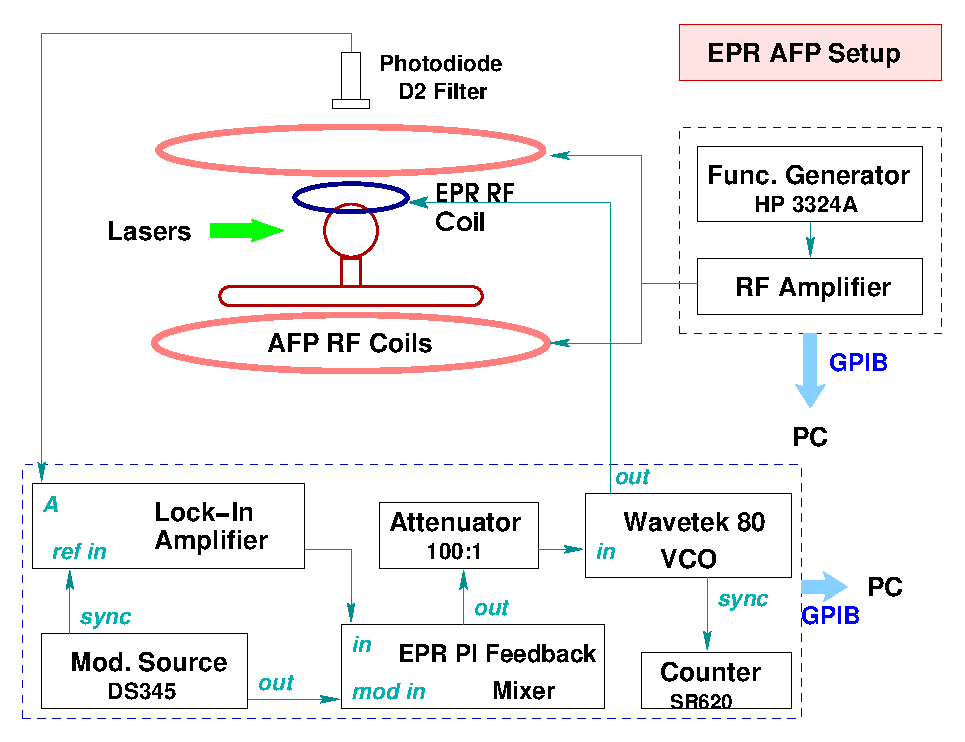
\includegraphics[scale=0.7]{eprfig2}}
%\caption{Circuit for EPR measurement with AFP spin flip}
%\end{center}
%\label{fig2:epr}
%\end{figure}
%
%
%Now that the circuit is built, you can begin the initialization of the
%setup.
%
%\begin{enumerate}
%
%\item Set the modulation source DS345 amplitude to approximately 0.6 Vpp.  
%This number can be optimized for different conditions such as different 
%target polarization and EPR D2 signal amplitude.  At an EPR D2 signal amplitude
%of 25 $\mu$V the optimized DS345 amplitude is roughly 0.05 Vpp for P$< 20\%$, 
%between 0.05 and 0.6 Vpp for $20\%<$P$<40\%$, and 0.6 Vpp or higher for 
%P$> 40\% $.
%
%\item Find the EPR resonance frequency:\\
%
%If you have done a FM Sweep measurement, then you already know the
%EPR resonance frequency, continue to the next step.\\
%
%If you don't know where the resonance frequency is, you may want to do 
%a FM sweep measurement, or you can 
%find the current resonance frequency by hand,
%To do this, 
%\begin{itemize}
%\item Temporarily remove the
%connection to Vin on the PI feedback box, turn off the integration
%function, set the 100:1 attenuator switch to ``FMS (short)''.  Now you are back to the FM Sweep circuit setup.
%Manually adjust the Wavetek 80
%frequency with the smallest step 0.01 MHz, 
%while observing the lock-in.  Look in the area
%given by the formula:                                                                                       
%
%EPR base resonance = (466000 * holding field in Gauss) 
%
%This is typically about 11MHz.
%
%\item You should be able to observe the lock-in signal changing 
%when adjusting the frequency.  It should show a maximum ($>$0, peak) followed
%by a minimum ($<$0, dip), or vice versa, and the resonance is between them
%when the lock-in signal is small.  Keep in mind that the lock-in will
%read zero when you are far from resonance
%as well, so be sure to look for this characteristic resonance behavior. 
%
%\item Reconnect the Vin input, and
%set the 100:1 attenuator switch from ``FMS (short)'' back to ``AFP (100:1)''.   
%\end{itemize}

%\item Set the Wavetek 80 frequency
%to be 0.1 MHz lower than the current resonance frequency if the light is
%right-handed polarized, or 0.15 MHz lower than the current resonance frequency 
%if the light is left-handed polarized.
%The lock-in signal should be large since you are not at the resonance frequency.
%
%\item Turn on the integration on the PI feedback box.
%
%\item Observe the Vout of PI circuit on an oscilloscope.  If it is ``jumping
%around'' erratically, or looks as if the  Opamps have been saturated, you
%must adjust the gains.  The best advice
%is to begin with the relative gain, and if this does not rectify the
%problem, move on to the absolute gain. 
%Basically, adjust these parameters such that the feedback signal is not too strong,
%neither too weak. \\
%
%\item Once this is done, the circuit should track
%the resonance frequency and the counter reading should change towards it.  The lock-in
%signal should be stablized to minimum.   
%
%\item Wait until the counter reading is stablized, change Wavetek frequency manually
%by 0.01 MHz.  You can observe a jump of 0.01 MHz in counter reading, but then
%it should change back to the resonance frequency, which means the circuit is following
%the resonance.  If not, then the frequency
%it was stablized before is not the true resonance frequency, check the circuit and
%try again.
%
%\item Once this is done, the circuit
%should take care of itself.  Left alone, it will track the movement of
%the resonance peak.
%\end{enumerate}        
%
%To measure the shift in resonance frequency due to AFP spin-flip, 
%open the LabView program AFPSweep.vi.  Enable the program by clicking
%on the large white arrow in the upper left corner of the panel.
%
%\begin{enumerate} 
%\item Set the sweeping time to be 6 seconds and the waiting time to be 20 seconds.  
%Set the number of sweeps to be 2.
%\item Run the program.
%\item Download parameters by clicking the corresponding button, you should read 
%``downloading parameters'' on the program status dialog.
%\item Wait until the program status shows ``waiting for data taking to start''.
%\item Start data taking by clicking the ``pause :: run'' button.  Now the program 
%should read resonance frequency from counter, and the lock-in amplifier signal.  
%The program status should show ``waiting for sweep trigger''.
%\item Wait for roughly 20 seconds, start sweeping by clicking on the ``start
%sweeping'' button. The program status should show ``sweeping...''.
%\item You should then be able to see the jump in resonance frequency.  When the light
%is right-handed polarized, this should be a positive jump, while for left-handed
%light it is negative.
%\item After the sweeping is completed, wait until the program status shows ``waiting 
%for sweep trigger'', now you can stop the program.
%
%\item Disconnect the output of Wavetek 80 to the cable leading to RF coil.
%
%\item \emph{Never stop the program during sweeping, this will cause the $^3$He
% to stay 
%at the wrong state and hence a big loss in target polarization. }

\item Refer to the circuit diagram. Start from the configuration as you were 
doing FM sweep.

\item Connect the lockin output from the back of the lockin to the INPUT of the PI box.

\item SET the GAIN to the number you have got from the FM sweep vi.

\item Open EPRAFP.VI

\item RUN it. SET the DEFAULT parameters. Frequency 78 to 92 KHz. 
V\_rms to 0.8 V.

\item Set it to MANUAL or AUTO. If AUTO, SET the wait time to 15 sec/20 sec.

\item POWER ON. You will see the frequency (GREEN) in the first plot, frequency fluctuation in the second plot and lockin signal in the third plot. Just dont worry about those at this moment.

\item SET the Integration gain at knob to 1 first in the PI box. Usually between 1 to 2 should be okay. But you have to play around. (The magic numbers we found is 1 to 1.2 for 100ms time constant and 1.5 to 1.7 for 200ms time constant)

\item TURN the INT GAIN ON in the PI box. You should see in the third plot 
the lockin signal approaching $0 \pm 5$ mV is okay. If not, try to increase the INT GAIN slowly till you feel comfortable.

\item WAIT for a couple of seconds.
  
\item START SWEEP. You should hear a ``click'' and see a drop or rise in the frequency (``well'' or ``hat'' shape) in the first plot.

\item If you are doing in MANUALLY, wait for 10 to 15 sec in that flipped state and hit ``START SWEEP'' again to get back to the original state. If you feel you need more data in that flipped state, wait for another 10 sec.

\item Repeat the above two steps one more time or two.

\item Make sure you end up in the original state. Then POWER OFF. SAVE the data. 
\item \emph{Never stop the program during sweeping, this could cause the $^3$He
 to stay at the wrong state and hence a big loss in target polarization. }

\end{enumerate}        

\begin{figure}
\begin{center}
\centerline{ 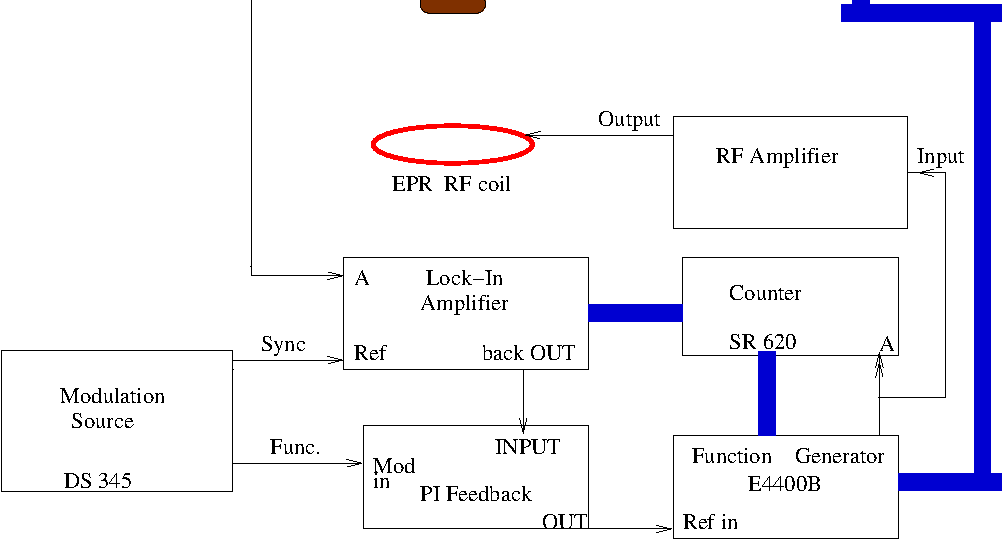
\includegraphics[scale=0.7]{eprafp}}
\caption{Circuit for EPR measurement with AFP spin flip}
\end{center}
\label{fig2:epr}
\end{figure}

\subsection{Common Problems}

\begin{enumerate}


\item The lock-in does not remain stable.  
Or the lock-in but does not seem to track the resonance.

You may see a big fluctuation in either lock-in signal or resonance frequency.
This effect can be caused by several things.  

First, it is possible that
the frequency to which you are locked is not the true resonance, or
you are completely out of resonance region.
The solution is again to find manually the resonance, looking for the
most pronounced signal.  

	The problem could also be caused by a wrong lock-in amplifier phase.
Please refer to Section \ref{sec:eprfms}.

	Finally, it could be that the PI Feedback box is improperly set. 
Adjust the gains until the lock-in becomes more stable.  
Admittedly this method is not very quantitative.
Based on experience, at high polarization ($>$40\%), both gains should be adjusted 
anti-clockwisely nearly to the end.  At lower polarization ($\sim$20\%), both gains should
be adjusted by about 4$\sim$5 turns clockwisely.
These numbers may also vary at a higher or lower EPR D2 signal amplitude.

You may also optimize the PI circuit gains by observing how fast the circuit 
follows the resonance.  When counter reading is stablized,
change Wavetek frequency manually by 0.04 MHz (which is close to the real jump
during sweeping, at a target polarization $\sim$ 40\%).  If the counter goes back 
to resonance in roughly 3$~$5 seconds, then the
circuit is working well.  If less than 2 seconds and counter reading is not stable, 
decrease both the relative and absolute gain.  If longer than 6 seconds or lose the 
signal, increase both the relative and absolute gain. 

\item The lock-in does not track the resonance when doing AFP flips.
This is common, since the frequency shift during the spin flip can be
quite large, on the order of 20-40kHz.  

	First, it is possible that the PI feedback is not strong enough for the circuit
to follow the resonance shift.  Try increasing the absolute gain of PI circuit
if possible.
	Second, it could be that the modulation DS 345 amplitude is too small.  The
size of this amplitude determines how far from the central frequency the circuit 
looks for the resonance.   Try increasing the modulation amplitude (but do not increase 
too much, usually it is less than 0.8 Vpp).  This will cause
the counter reading less stable and you need to compromise between stablizing the
circuit and following the frequency shift.


\end{enumerate}


%\subsection{EPR Continuous Monitoring with Field Feedback}  
  
%This configuration uses the lock-in amplifier with PI feedback 
%circuit to lock into the EPR resonance frequency and then track its
%behavior. At the same time a field feedback system is used to stablize the
%main holding field to a level of 10$^{-5}$.  The EPR resonance frequency is the central
%frequency proportional to the main holding field plus (or minus) a field originated
%from the $^3$He polarization.  By measuring the EPR resonance frequency and
%the main holding field, one is able to monitor the pumping cell polarization continuously.\\


%The circuit and labview program are the same to that are used for AFP Sweep 
%measurement described in Section \ref{sec:eprafp}, except that field feedback system 
%is needed, as shown in Fig. \ref{fig3:epr}

%\begin{figure}
%\begin{center}
%\centerline{ 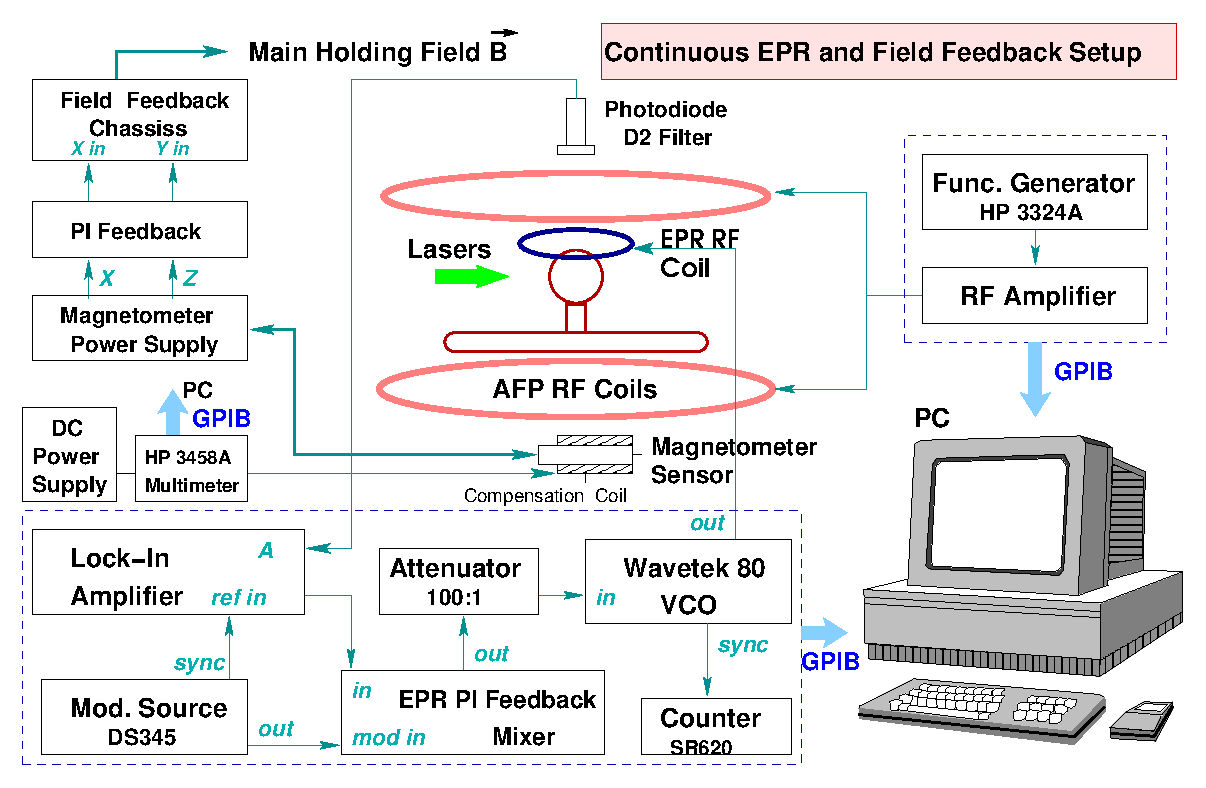
\includegraphics[scale=0.7]{eprfig3}}
%\caption{Circuit for continuous EPR measurement with field feedback}
%\end{center}
%\label{fig3:epr}
%\end{figure}



%\begin{enumerate}
%\item Construct circuit and set parameters.  To track the resonance frequency,
%the only difference between EPR AFP measuremen and EPR continous monitoring is 
%that the modulation source DS 345 amplitude does not need to be large.  Typically 
%0.05 Vpp is enough.

%\item Make sure the circuit is tracking the resonance frequency.

%\item Use a scope or multimeter to measure the two field feedback signals, the 
%amplitude should be less than 500 mV.  If either of them is larger than 500 mV, 
%you must adjust the position of magnetometer sensor such that the signal perpendicular
%to the main holding field is back to 200 mV or lower.  Then adjust the
%power supply for the compensation coil such that the signal parallel to
%the main holding field is back to 200 mV or lower.
 
%\item Enable the field feedback system by setting the switch 'bypass/through' 
%on field feedback chassiss to 'bypass'.  You should observe that both field 
%feedback signals are stablized to zero.

%\item Run LabView program HP3458A\_read.vi on computer downstairs to record the current
%of compensation coil.

%\item Open LabView program AFPSweep.vi, enable the program by clicking the
%white arrow in the upper left corner.

%\item Set the paramters, download parameters
%and start data taking.  Do not do sweeping (AFP spin flips).

%\item After enough data is collected, stop the program.
%
%\item Disconnect the output of Wavetek 80 to the cable leading to RF coil.
%
%\end{enumerate}



%\subsection{Common Problems}
%\begin{enumerate}
%\item See the problems in the previous section.

%\item The field feedback signals jump to +10V or -10V when enabling the field feedback
%system, and stay there afterwards.

%This is usually caused by a wrong state of the field feedback system.  For example, wrong
%sign of the feedback settings (XCOS, YCOS) can cause a positive feedback such that the 
%signals are stablized to the satuated values.

%\item The field feedback signals oscillate between +10V or -10V when enabling the field feedback
%system.

%This is also caused by a wrong state of the field feedback system.  Because we are using
%two dimensional field feedback, wrong
%sign of the feedback settings (XSIN, YSIN) will cause the longitudinal and transverse 
%components of the field interfering with each other through a positive feedback so both
%are not stablized.

%\item The field feedback signals are stablized at a small but non-zero value.

%This means the field feedback system is working properly and in principle should not
%affect the measurement.  However, a non-zero offset of either of the signals may cause
%a non-linearity between holding field and the compensation coil current, which should
%be avoided in high precision polarization measurements.  With the field feedback 
%system in `Bypass' mode, you can adjust the screws on 
%field feedback chassiss to adjust the `XOFFSET' and 'YOFFSET',
%meanwhile use a scope to measure the two field feedback signals from magnetometer sensor
%until they are stablized to zero.

%\end{enumerate}

} % infolev

\infolevone{
%===============================
%\chapter
\section{Reference Cell}
\label{sec:refcell}

\subsection{Description of the Reference Cell System}

The reference cell system is comprised of three subsystems---the
reference target cell, the gas handling system, and the control
electronics.  The reference target cell is mounted inside the target
enclosure, which is located in the beam path immediately upstream of
the spectrometers.  The gas handling system consists of a gas
manifold, which is located in the electronics rack near passageway under 
beam line, and a series of gas lines that connect the manifold to the
reference cell. A control box consisting of electronics that control
the solenoid valves of the gas system is also located in the
electronics rack.  A remote control box, identical to the one in the
hall, is located in the counting house.  A schematic of the entire
system is shown in Fig. \ref{fig:refcell1}.  The individual subsystems
are depicted in Fig. \ref{fig:refcell2}--\ref{fig:refcell3}.

\begin{figure}
\begin{center}
\centerline{ 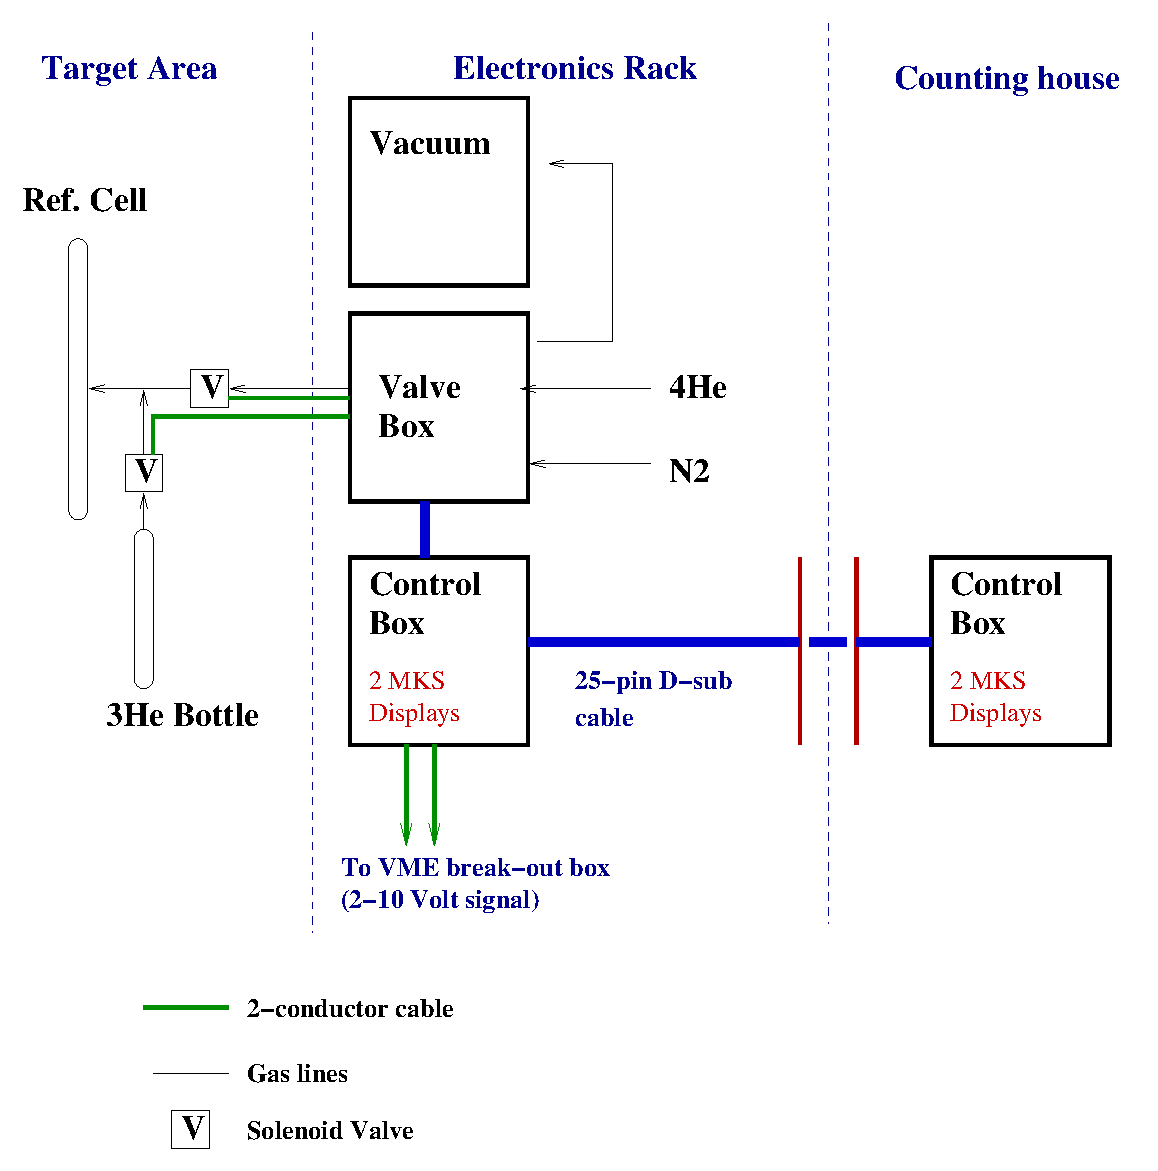
\includegraphics[scale=0.6]{ref_2}}
\caption{Schematic of reference cell system}
\label{fig:refcell1}
\end{center}
\end{figure}

Under normal operating conditions, the manifold, the reference cell,
and the intervening gas lines will be filled with either H$_2$, $^3$He,
or N$_2$ gas at high pressure 
(typically $\approx 10$~atm).  The system
may be operated either locally (at the panel) or remotely (via
switches mounted in the counting house).  A switch on the
remote gas panel itself allows one to toggle between local and remote
control.  All switches, local and remote, are equipped with LED
displays so that one can readily determine the status of any switch.

The reference cell consists of a very thin-walled glass flask.  An
outlet at the opening is joined to a Copper tube by means of a
glass-to-metal seal.  This Copper  tube is connected to a 1/8" dia.
Copper tube with quick-plug-on gas fittings. High pressure $^3$He gas
bottle is mounted near the target chamber and is connected to the
other end of the 1/8" Copper tube through solenoid valve {\bf V3}. The
rest of the gas system is connected to the 1/8" copper tube by a long
1/2" Copper tube. The reference cell is mounted at the gas fitting. A
special coupling tool has been designed to facilitate the
coupling/de-coupling the reference cell at the quick-plug-on gas
joint.

The gas handling system consists of 7 solenoid-controlled,
air-actuated valves, one hand-set needle valve, two baratron pressure
gauges (0--1000 torr and 0--1000 psia), two pressure relief valves, a
bottle of high-pressure $^3$He gas, a bottle of high pressure N$_2$
gas, a bottle of high pressure H$_2$ gas, an oil-free MD pump
backed up by a backing pump, and sufficient tubing and pipe fittings to
connect them all together.  There are 5 basic actions that the gas
handling system must accomplish; pump-out, vent, fill with H$_2$, N$_2$, or 
fill with $^3$He. 

The reference cell control panel (shown in Fig.~\ref{fig:refcell3} )
is comprised of 5 pushbutton switches, which activate the 5 possible
valve setting conditions, a baratron high-pressure gauge which reads
between 0-1000 psia, a baratron low-pressure gauge which reads between
0-1000 torr, two toggle switches to turn on and off the vacuum pump
and a toggle switch to select local or remote operation.  The valve
configurations for the five actions are described in
Table~\ref{tab:refcell}.

\begin{table}
\begin{center}
\begin{tabular}{|c|l|c|}
\hline\hline
Condition & Action & Valves activated (open) \rule[-2.5mm]{0mm}{7mm}\\
\hline
C1 & {\bf Evacuate} & V1+V4+V5 \\
C2 & {\bf Vent} & V4+V5+V7 \\
C3 & {\bf $\bf ^3$He fill} & V3 \\
C4 & {\bf N$\bf _2$ fill } & V2+V4+V5 \\
C5 & {\bf H$\bf _2$ fill } & V4+V5+V8 \\
\hline\hline
\end{tabular}
\caption{Action of the remote-control switch panel}
\label{tab:refcell}
\end{center}
\end{table}
\begin{figure}
\begin{center}
\centerline{ 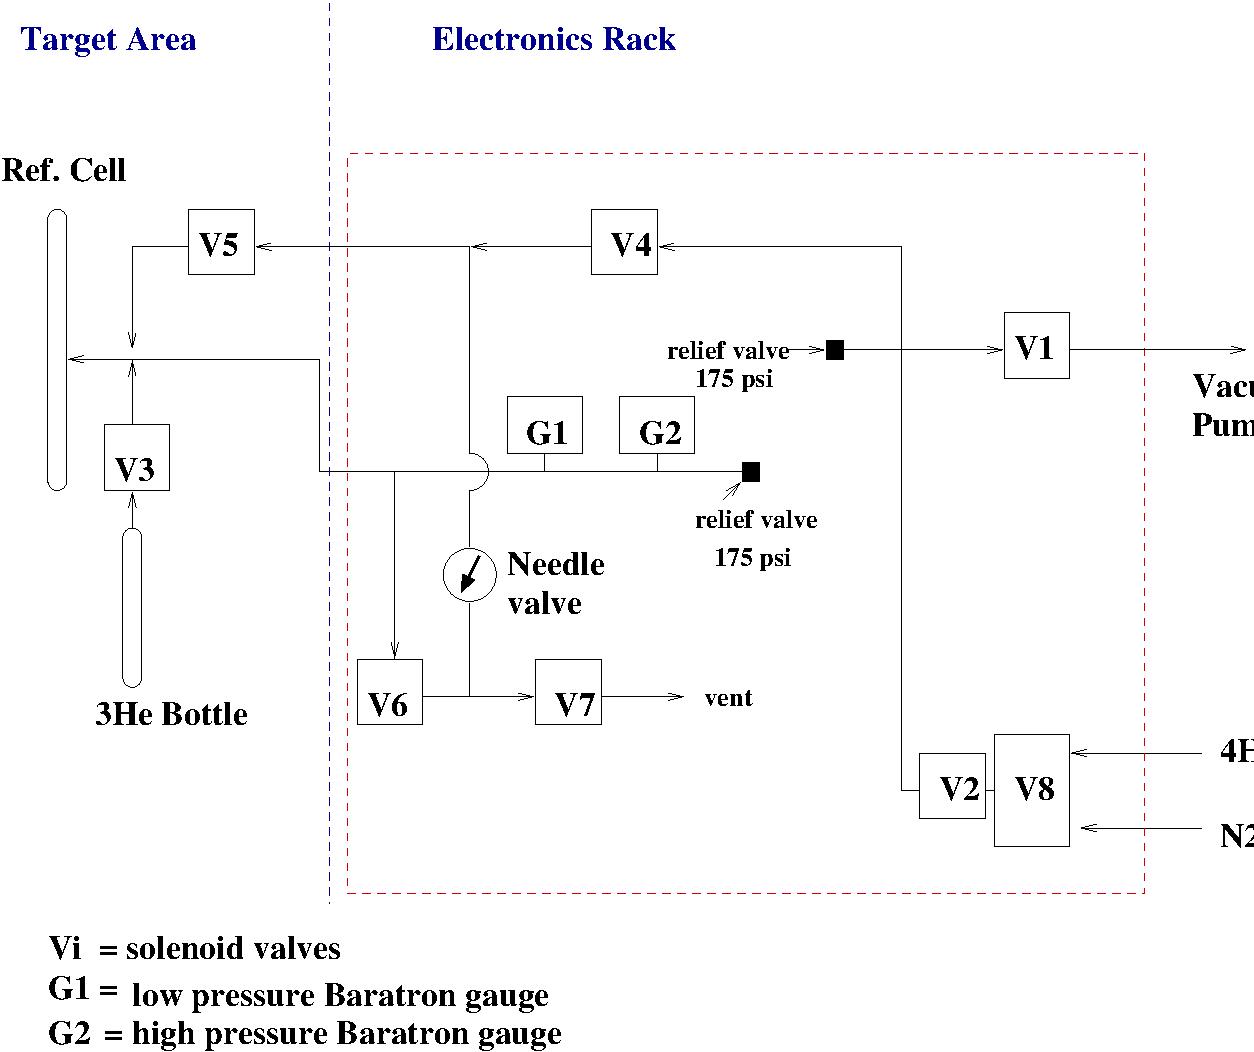
\includegraphics[scale=0.6]{ref_panel}}
\caption{Valve configuration of the reference cell gas system}
\label{fig:refcell2}
\end{center}
\end{figure}

\begin{figure}
\begin{center}
\centerline{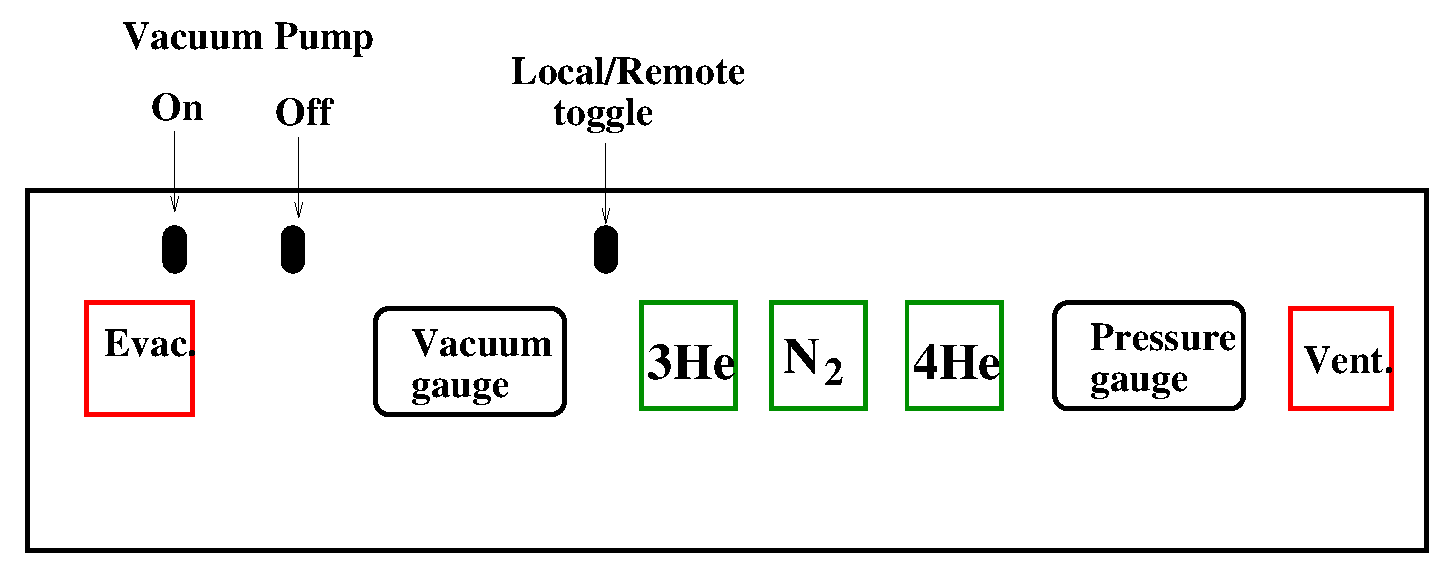
\includegraphics[scale=0.6]{ref_3}}
\caption{Control panel}
\label{fig:refcell3}
\end{center}
\end{figure}


\subsection{Operation}



The following operational sequences will allow the filling of the reference cell with the three gases:

\begin{itemize}
\item Fill with N$_2$
\begin{itemize}
\item Step 1: Vent to 16 psia.
\item Step 2: Evacuate until vacuum reaches 1 mtorr.
\item Step 3: Hold the N$_2$ button down while checking the high-pressure gauge, until the desired pressure is established.
\item Repeat steps 2,and 3 three times.
\end{itemize}
\item Fill with H$_2$
\begin{itemize}
\item Step 1: Vent to 16 psia.
\item Step 2: Evacuate until vacuum reaches $< 10$ mtorr.
\item Step 4: Hold the H$_2$ button down while checking the high-pressure gauge, until the desired pressure is established.
\item Repeat steps 2, and 3 three times.
\end{itemize}
\item Fill with $^3$He
\begin{itemize}
\item Step 1: Vent to 16 psia.
\item Step 2: Evacuate until vacuum reaches $< 1$ mtorr.
\item Step 4: Hold the $^3$He button down while checking the high-pressure gauge, until the desired pressure is established.
\end{itemize}
\end{itemize}




The pressure at the location of the gas
manifold is measured by a  baratron gauge.  The baratron
pressure is read into the data stream and is also output to a remote
sensing unit located in  the counting house.




\subsection{Cautions}
\label{sec:targ-hel-saf}

\begin{enumerate}

\item Be careful with the $^3$He, we have a limited supply.

\item If the system is above atmospheric pressure, always vent it
before pumping.  

\item Always monitor the high-pressure gauge when filling. Do not  exceed 150 psia.

\end{enumerate}

\begin{safetyen}{10}{5}

\subsection{Potential Hazards}

The principal hazards associated with the reference cell are
flying material and loud noise if the gas panel or reference cell
fails catastrophically under high pressure.  Of the two subsystems,
the reference cell subsystem presents the greater hazard, both because
it is more likely to fail, and because it is likely to be more
dangerous if it does.  The target enclosure is designed to contain all the 
debris in case of a cell explosion.


\subsection{Hazard Mitigation }

After testing the reference cell system to 200 psia and to protect the
cell from rupturing during normal operation, the relief valves have
been set to 175 psia.


All personnel shall wear hearing protection when accessing the
 platform area while the cell is under high pressure and no windows
 are on the target enclosure.

Special care must be taken when accessing the region inside the target
enclosure.  Full face shielding and safety glasses should be worn
under these conditions.  Before working in the vicinity of any of the
reference cell components, personnel shall check the pressure in the
manifold from the baratron readout in the remote control area.

\end{safetyen}

} % infolev
%====================================================
%\chapter
\begin{safetyen}{10}{5}
\section{Hazards and Safety Issues}
\label{sec:haz}

The main potential hazards encountered in the overall operation of the
target are listed below.
As we address the operation of each subsystem, a description on how to
alleviate the potential
hazards is reported. 

\begin{itemize}
  \item Personnel eye sight damage due to exposure to infrared laser light;
  \item Fire due to the operation of the high power lasers;
  \item Fire due to the operation of the target oven;
  \item Explosion of the high pressure target cell;
  \item Explosion of the reference cell;
  \item Activation of the target caused by the electron beam.
\end{itemize}

For personnel safety to be effective all personnel authorized to operate
any subsystem of the target will be required  be familiar with that 
specific subsystem as well as read 
\infolevone{this} \infolevltone{the full} target OSP% 
\infolevltone{~\cite{HallAosp}}.

A target operator is on shift usually when the target laser system is on.
A training session is required of any target operator. 

\end{safetyen}

\begin{safetyen}{10}{5}
%======================================================
%\chapter
\section{Laser Safety}
\label{sec:lsafe}

\subsection{Laser Safety}
\label{sec:lassaf}

\begin{enumerate}
\item Always have your safety goggle on when the laser is on!
\item When the yellow beacon is flashing, have goggle on when you enter
the hut.
\item Alignment should be done at low power.
\item Be sure that the beam is hitting the target.
\item Do not turn the beam up to full power unless the oven temperature
is at least 150 degrees Celsius.
\item Do not look directly into the beam even with safety goggle on.
\item Do not stand in the way of a beam that is at full power.
\item Understand where the beam is and where the reflections are.
\end{enumerate}

\subsection{Fire Hazards and Safety}
\label{sec:targ-polhelfire}

The fire and safety in the laser room is covered in the LOSP
for the laser room,
however, in the target area where the laser beam is directed, there is a
case where a potential 
fire hazard exists. 

In case the target cell explodes during optical pumping, the temperature 
sensors mounted on the target and pumping cells will respond immediately and 
an alarm will be triggered. The alarm will be triggered whenever 
a temperature reading of any sensor is 10$\%$ out of its norminal range.
The target operator should shut off all the lasers immediately.
Based on the tests performed, the target oven will sustain on the order of 10 
minutes with full laser power incident and no rubidium atoms 
to absorb the laser power.


\subsection{Personnel Safety/ Working in the Hall}
\label{sec:prs}

When the installation of the full target setup is finished, working in
the hall
shall be safe from laser light hazards or target explosion hazards,
because 
laser light as  well as the target cell will be safely enclosed.
Therefore 
when considering the overall aspects of the safety of personnel working
in the
Hall two distinct periods are to be considered.

\begin{enumerate}

\item One period is during the laser beam alignment because the laser
beam pipes
from the laser hut to the  target need to be removed. During this time
period we
will ensure that no other person except those people who are laser
trained are in the hall. This will be arranged by using a
controlled access 
to the Hall provided by the CANS system.
This alignment 
will be performed usually during the night time and (or) weekend. 
Clear warning signs will
be posted  at the
entrances of the Hall when the alignment is under progress.

\item One period is during the setup of the high pressure target cell in
its final position, or when replace a target cell, or perform target related 
work requiring opening the enclosure.
In this case the ``target platform'' which is a natural perimeter around
the target area 
 will be marked  and signs posted requiring the wearing of ear
protection and
faceshield. Lasers should be tuned off and fibers be disconnected and locked 
away following the lock-and-tag procedure.
Beyond that defined perimeter all personnel working in the
hall
will not be affected in case of explosion of the cell if they are not 
wearing  a faceshield. Nevertheless, it is strongly recommended to have 
ear protection when working anywhere in the Hall. 
\end{enumerate}
\end{safetyen}

\infolevtwo{
%----------------------------------------------
%%% LSOP...
\section{Appendix: Laser Standard Operation Procedure}
\label{sec:lsop}

\subsection{ Introduction}

A polarized $^3$He target system was built and used for several 
JLab experiments. A number of new experiments will continue use the 
polarized $^3$He target system in the future. 
The polarized $^3$He target is based on 
the principle of spin exchange between optically pumped vapor of Ru-K mixture 
and $^3$He gas. Several high power (30 Watts) 795 nm diode lasers will be used 
for the optical pumping. A laser room outside the hall is built to house the 
lasers.
This LSOP describes the setup of the 
laser system in the laser room and at the target area, 
details the potential
hazards associated with the operation of this setup and provides instructions
for the safe and effective use of the equipment. In addition,
this manual provides information about the functioning of the various safety 
systems installed to protect personnel and equipment.

\subsection{Personnel and Required Training}
\label{sec:target-phe3-laser-train}

The 30 watts infrared diode lasers (Coherent FAP-System and Newport Comet lasers) may only be operated by
personnel who have :
\begin {itemize}
\item completed a Laser Safety course administrated by the laser safety officers at
Jefferson Laboratory (Bert Manzlak).
\item read the Laser Safety section of the EH\&S Manual(6410);
\item  completed and passed an opthalmological exam;
\item had a safety walkthrough by the Laser Safety Supervisor of the 
Polarized $^3$He Target System (Jian-ping Chen);
\item read this document;
\item been added to the authorized list of Laser Personnel, included as the 
last page of this LSOP.
\end {itemize}
Jefferson Lab personnel or outside visitors, who have not completed all of 
above training, are
only allowed to enter the laser control area under the following conditions :
\begin {itemize}
\item have permission of the Laser Safety
Supervisor of the Polarized $^3$He target system
\item be accompanied by a laser authorized personnel
\item if the laser is operational, with required safety
goggles
\item if any equipment, including the laser, is operational, no touching of
equipment due to electrical hazards.
\end {itemize}


\subsection{Laser}

The main Laser specifications are outlined in Table~\ref{tab:coherent} and
Table~\ref{tab:Comet}. For more specific
information, we refer to the Coherent FAP-system diode laser users manual
and the Newport Comet diode laser manual, 
which will be available in the lab.

\begin{table}
\begin{center}
\begin{tabular}{|l|l|}
\hline
& \\
{\bf Specifications}&{\bf COHERENT FAP-System} \\
\hline
& \\
\underline {\it Operational Specifications}& \\
Output power			& 30 W \\
& \\
\underline {\it Mechanical Specifications}& \\
Weight			        & 60 pounds  \\
Cooling Requirements 		& None required \\
Delivery Optical Fiber Bundle   & 0.8 mm diameter \\
Delivery Fiber Length		& 5.0 meter nom.\\
Delivery Fiber Termination	& SMA 905 conn. \\
& \\
\underline {\it Operational Specifications}& \\
Typical Operating Temperature   & $0^\circ$C to $35^\circ$C \\
Typical Storage Temperature     & $-20^\circ$C to $65^\circ$C \\
Humidity (non-condensing)       & $5\%$ to $95\%$  \\
& \\
\underline {\it Electrical Specifications}& \\
Input Power	                & 115 Vac 60 Hz, $<1200$ W (500 W typical) \\
& \\
\underline {\it Optical Specifications}& \\
Beam Characteristic 		& Semiconductor, multimode \\
Beam Divergence        & $<0.20$ N. A. \\
Diode Laser Center Wavelength   & 780 to 840 nm \\
Wavelength Temp Coefficient	& 0.27 to 0.30 nm/$^\circ$C \\
Emission Bandwidth (FWHM)       & $\pm 2$ nm \\
\hline
\end{tabular}
\label{tab:coherent}
\caption{Coherent laser specifications}
\end{center}
\end{table}

\begin{table}
\begin{center}
\begin{tabular}{|l|l|}
\hline
& \\
{\bf Specifications}&{\bf Newport Comet Diode Laser System} \\
\hline
& \\
\underline {\it Operational Specifications}& \\
Output power			& 30 W \\
& \\
\underline {\it Mechanical Specifications}& \\
%Weight			        & $<60$ pounds  \\
Cooling Requirements 		& None required \\
Delivery Optical Fiber Bundle   & 0.4 mm diameter \\
Delivery Fiber Length		& 1.0 meter nom.\\
Delivery Fiber Termination	& SMA 905 conn. \\
& \\
\underline {\it Operational Specifications}& \\
Operating Temperature   & $20^\circ$C to $35^\circ$C \\
Storage Temperature     & $-30^\circ$C to $50^\circ$C \\
Operating Humidity        & Non-condensing  \\
& \\
\underline {\it Electrical Specifications}& \\
Input Power	                & 115 V, 60 Hz, 6 Amp max. \\
& \\
\underline {\it Optical Specifications}& \\
Operating Cionditions 		& standard CW \\
Beam Divergence        & $98\%$ within 0.22 N. A. \\
Diode Laser Center Wavelength   & 794.69 nm \\
Temperature Tuning	& 0.005 nm/$^\circ$C \\
Spectra Width (FWHM)       & $\le 0.35$ nm \\
\hline
\end{tabular}
\label{tab:Comet}
\caption{Comet laser specifications}
\end{center}
\end{table}

\subsection{Optical setup}

The optical setup is shown in Fig.~\ref{fig:optics_setup}, and is made of:
\begin {itemize}
\item Up to 15 infra-red diode lasers (five for each pumping direction) 
located on two racks in the laser room;
\item Fifteen long (75 m) optical fiber to transport laser beam from the lasers
into the hall;
\item Three 5-to-1 optical fiber combiners, one for each pumping direction;
\item Six lens, two lenses for each laser beam to have it focused at the 
pumping cell;
\item Three beam splitters to split each laser beam to two beams with linear polarization;
\item Nine $\lambda$/4 waveplates, six with rotating motors, to transform 
each beam from linear polarization to right or left circular polarization;
\item Twelve dielectric mirrors to reflect each split beam back into the pumping cell;
\item Three transparent windows 
on the oven to allow the combined laser beams to pass through;
\item One pumping cell to absorb all the laser beam power;
\item One mirror and three optical fibers with lenses for 
spectral-analyzer and for EPR;
\item One spectral-analyzer for monitoring the pumping cell.
\end {itemize}

For each pumping direction, up to five diode lasers will be used. 
After passing through the 75 m long fibers, they will be combined
to be one beam with a 5-to-1 optical fiber combiner. The combined beam, after passing through two lenses,
will be split into two beams. Each one will go through a $\lambda$/4 waveplate
to transform linear polarization to circularly right or left polarization. 
All beams, after passing some windows and being reflected by some mirrors,  
will shoot into a glass pumping cell filled with
mixture of Rb-K vapor and $^3$He gas. The laser beams will be mostly absorbed
by the pumping cell. The total path length from the output of 5-to-1 combiner 
to the pumping cell
is about 5 meters. The pumping cell is inside an oven and 
connected to a target cell. The whole target assembly is inside three pairs of
Helmholtz coils, which provide a magnetic field for the polarization of the
target. A NMR system with a set of RF drive coils and a set of separate 
pickup coils, and an EPR system 
are used to measure the polarization of the target.


\subsection{Hazards}

The primary beam hazards associated with Class IV lasers consists of eye and skin
injuries. The most severe eye injuries are caused by viewing the beam either directly
or through specular reflection. At an infra-red wavelength of $795 nm$ most of the
laser light entering the eye is absorbed in the retina. The primary adverse effects
from direct or specular viewing are blindness and severe retinal burns. The primary
adverse effects from accidental viewing are retinal burns. The retina is most
sensitive to radiation of this wavelength, and if the laser energy incident to the eye
is too high, it can cause an irreversible retinal burn.

Laser radiation of the intensity associated with Class IV diode lasers can also
cause irreversible damage to the skin. The damage caused is either associated with
temperature rise of the skin tissue following the absorption of laser energy (skin
burns) or with surface reactions resulting from photon interactions at the molecular
level (photochemical effect), disrupting the normal functionality of the skin tissue.

The normal Hazard Zone for the 30 Watts FAP system is $2.76 \times 10^3$ meters.


\subsection{Laser environment}

The diode lasers and the associated devices will be located in the
laser room outside Hall A.  The entire laser room is a
laser controlled area (see Fig.~\ref{fig:laser_newroom}).

\begin{figure}
%  \begin{center}
  \centerline{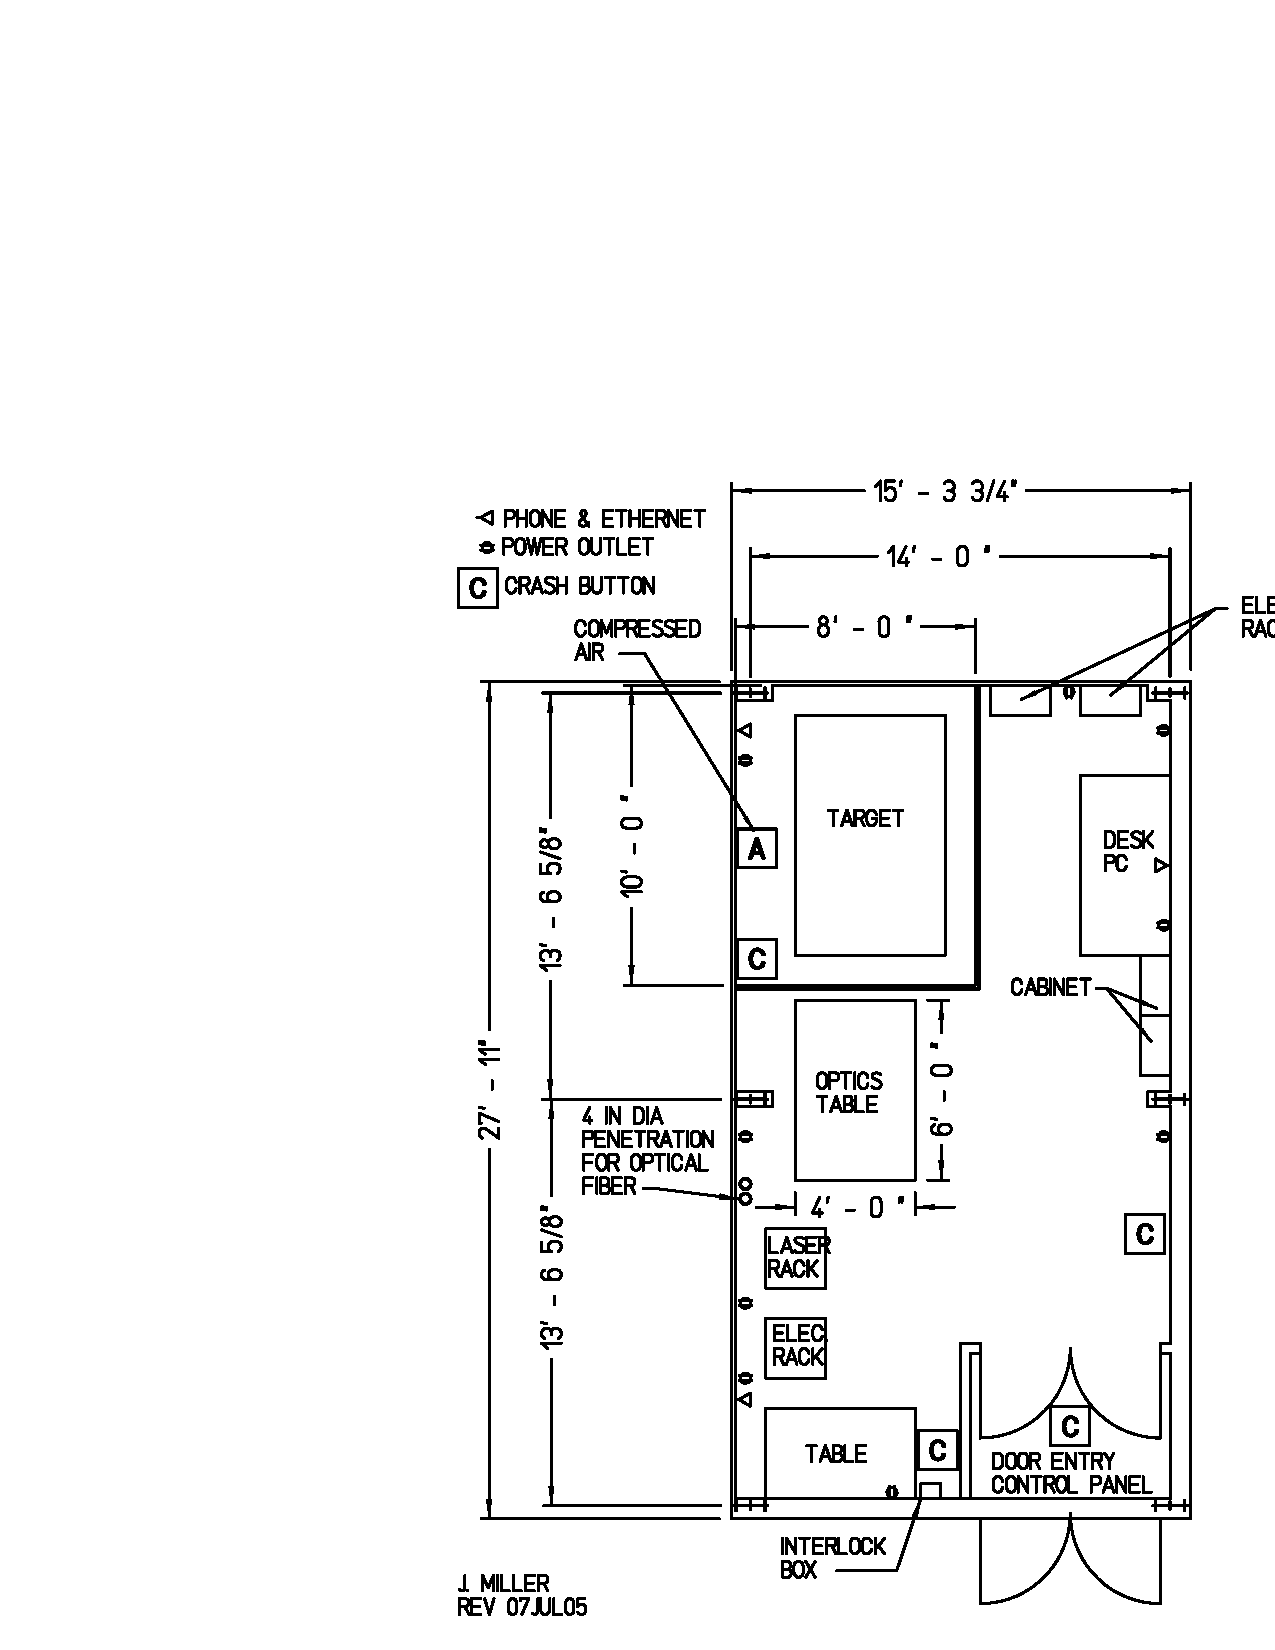
\includegraphics[width=\textwidth]{laser_newroom}}
  \caption[Polarized $^3$He Laser Room Layout]{The Polarized $^3$He Target 
Laser Room Layout}
%  \end{center}
   \label{fig:laser_newroom} 
\end{figure}

Laser beams go into the hall via long optical fibers
and then combined to form desired polarized lights for optical pumping.
The setup is shown in Fig.~\ref{fig:optics_setup}.
After passing through the optical setup, the laser beams 
are directed into the pumping cell and terminated there. 

\begin{figure}
%  \begin{center}
  \centerline{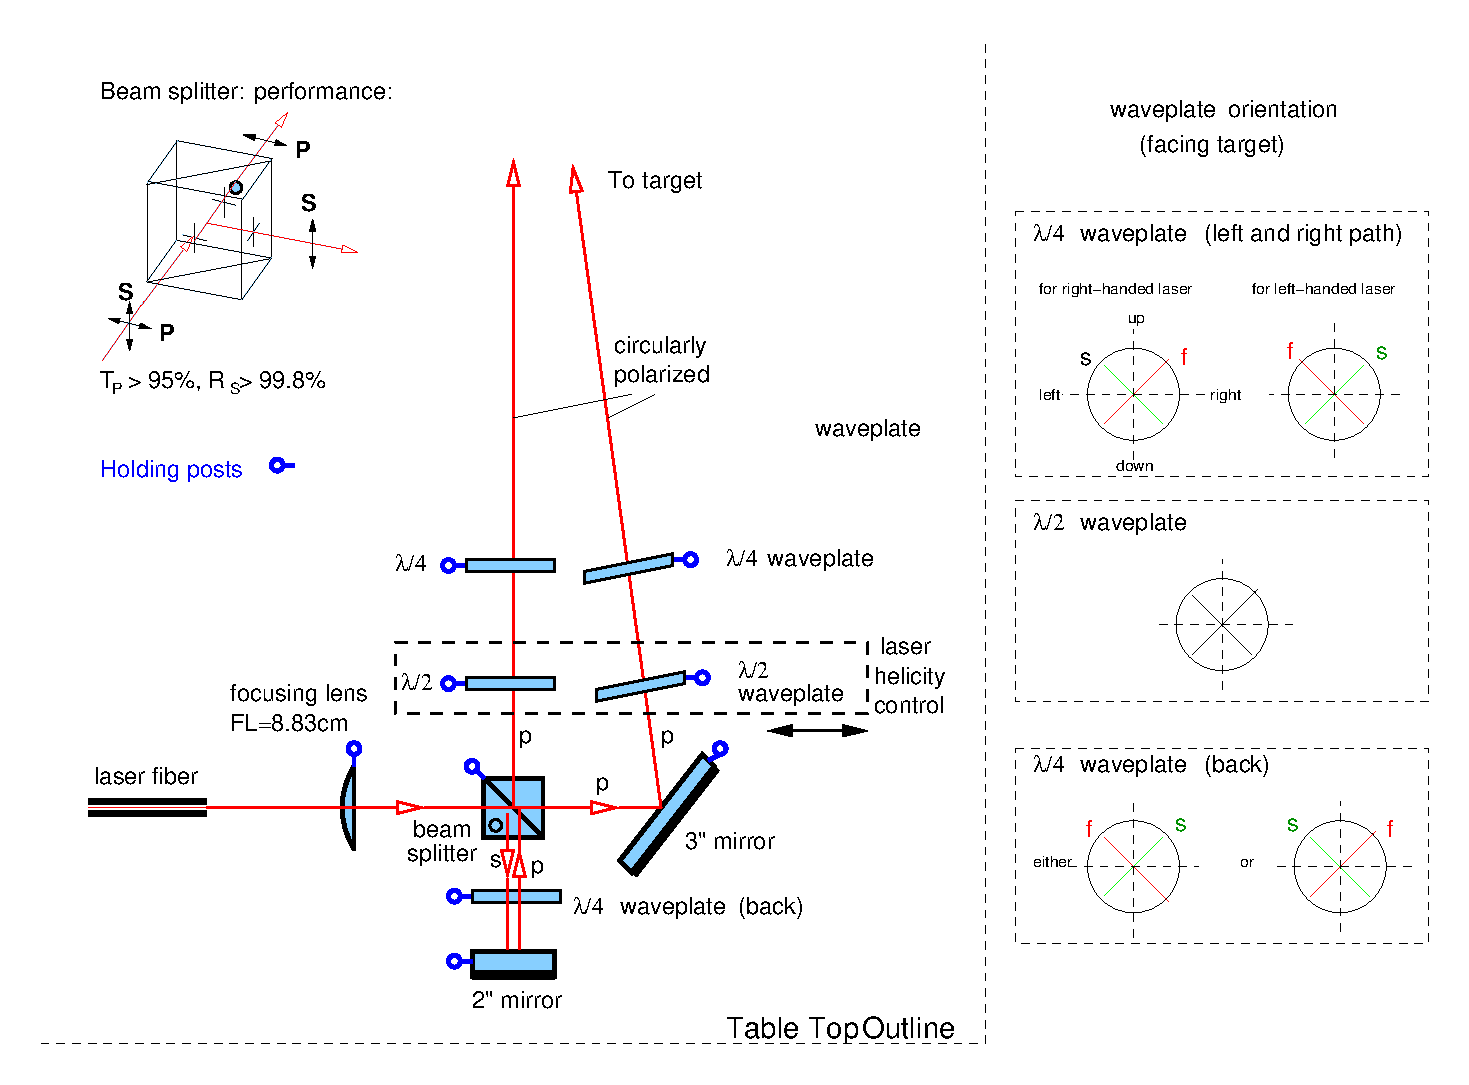
\includegraphics[width=\textwidth]{laser_setup}}
  \caption[Polarized $^3$He Laser Optics Setup]{The Polarized $^3$He Target 
Laser Optics Setup}
%  \end{center}
   \label{fig:optics_setup} 
\end{figure}


Outside the laser room, the laser beam path is completely enclosed with beam 
pipe between the laser room and the target pivot and an enclosure on top of the 
the target. 

Apart from direct beam hazards to eyes and skin, since the diode lasers are 
Class IV lasers, there exists a potential fire hazard. Flammable material 
should not be brought into the laser area.  

\subsection{Procedures}

In this section, we review the various procedures that are required to operate the
laser and optical devices. Hazards are least likely to occur during normal operation
when laser beams are switched on. During tests, maintenance,
upgrades and/or alignment,  beam hazards are more likely.

{\bf At all times}, when operating the diode lasers in lasing mode, safety goggles
are required.

\subsubsection{Normal procedure}
In the operation mode, each diode laser is in lasing mode rendering an output 
power of approximately 30 W. The laser beam is already aligned, properly 
focused and directed into the pumping cell. The lasers are interlocked with the
entrance door of the laser hut. All the laser beam pipes and the laser 
enclosure on top of the target are securely installed.

Working with the lasers in normal operational mode will require protective 
eye wear with a minimum optical 
density (OD) of 4.7 at wavelength of 795 nm. Before
starting the laser in its normal operation mode personnel have to enable the
laser safety interlock box. This will cause access to the laser room to be in 
a controlled mode. Authorized personnel with an access code can 
bypass the interlock for 45 seconds when entering the laser room. Unauthorized
personnel entering the room will cause the lasers switching to stand-by mode
when the door is opened. If the laser is to be unattended for a long time, the 
power should be switched off.

Thus the general procedures for normal operation of the diode lasers in the target lab are:

\begin {itemize}
\item Enable laser safety interlock box;;
\item Wear protective eyewear;
\item Switch on AC power;
\item Turn on the control box with a key; 
\item Turn laser to Ready and then On.
\end {itemize}

\subsubsection{Alignment procedure}

All the mechanical stands supporting the optical components have been
designed and surveyed in order to achieve a preliminary safe alignment
of the entire setup (laser off).  Initial setup of laser and optical
system will be done while the laser hut window is closed (such that no
laser beam will come out the laser hut).  Initial alignment will be
done with a standard class 3 HeNe laser (class 3A after attenuation,
650 nm) or a laser pointer (class 3A).  Laser safety goggles are
mandatory for all procedures except for alignment using class 3A HeNe
laser. Use precaution for class 3A laser when using the HeNe laser: Do
not look directly into the beam or use collecting optics.  The final
alignment will be done with the diode laser but at a reduced laser
power (less than 10 amps, when the laser spot on a card can be clearly
seen with IR viewer). The alignment is performed with one laser beam
line at a time.  The beam can be tracked by the use of either an IR
viewing card or an IR viewer.  The photosensitive card can be
displaced along the beam, and the IR viewer allows the tracking by the
light slightly diffused on the optical components. During this final
alignment, the laser hut window will be opened and the laser beam will
be directed to the target, while the laser beam pipes and the laser
enclosure on top of the target will be taken off. Therefore the whole
hall will be classified as laser area. We will use the CANS system to
have controlled access. Before the laser alignment starts, a sweep
will be performed to clear the Hall. Then the CANS system will be
programmed to only allow authorized laser trained persons to have
access to the hall.  The door to the BSY tunnel will be magnetically
locked with a toggle push-button switch. The ``laser danger'' warning
sign will be posted at all the entrances. The doors will be checked by
pulling the door handle. In addition, a red flashing light will be put
at the BSY side of the door.
%key-interlock 
%entrance control system to have controlled access. Before the laser alignment
%starts, a sweep will be performed to clear the hall. Then the hall will be in 
%``control access'' mode. MCC will only allow authorized laser trained persons 
%to have access to the hall. A copy of this LSOP with a current list of 
%Authorized Persons will be kept at MCC. 
Most of the final laser alignment will be performed during night time
to minimize interference with other work going on in the hall. When
the alignment stops, all signs will be take off and the CANS system
will be disabled and the door to BSY will be unlocked.

\subsubsection{Maintenance procedure}

Replacement of used or damaged optical components of the setup will be made with the
laser off (power switched off and unplugged).  The positions and 
orientations of the new components will be mechanically
surveyed and extensively checked before turning to any procedure needing the laser on.

When the target enclosure windows need to be opened (such as to inspect
the target or to replace a 
target cell) and the hall is not in laser controlled access, 
the lasers must be turned off before opening the target enclosure.
The 
keys for all of the laser power supplies 
optical fibers will be disconnected and the connection ends
will be secured in a lock box.  All staff working in the
vicinity of the target enclosure 
must apply personal locks to this box in accordance with
JLab lockout/tagout procedures.
The vicinity area will be determined
from the power measurement and with clear danger sign posted.

In case of the failure of any electromechanical or electrical or electronical device,
the lasers and the other power supplies will be turned off. The Laser power
can simply be unplugged.


\subsubsection{Off-normal and emergency procedure}

In case of an emergency, power to the laser should be shut off.
This can be performed in three ways.
\begin {itemize}
\item Push the Crash button;
\item Turn off the control key on the laser power supply;
\item Pull the plug from the power outlet.
\end {itemize}

In the event of a fire, the users should leave the laser room and pull the 
nearest fire alarm. Then leave the hall.

In case anybody is accidentally exposed to the laser beam (direct or indirect)
without eye protection, he or she should immediately contact the Jefferson
Lab medical center (phone: 7539, page: 584-7539). If it is 
off business hours, please contact local hospital emergency. At the mean time,
please inform the laser system superviser (Jian-ping Chen, phone: 7413,
page: 584-7413) and/or laser safety officer (Bert Manzlak, phone: 7556,
page: 584-7556). 


\subsection{Controls}

Several controls have been added as preventive measures to the laser room 
and to the direct laser area. We will enumerate these controls here.
\begin {enumerate}
\item The laser control area will have danger signs posted and will have a
yellow beacon indicating the presence of Class IV diode lasers. Danger
sign will also be posted near the target enclosure area.
\item A controlled access interlock system will limit the entrance to
the laser room with a coded number pad. The code is given only to the
authorized laser users listed in section 10 with currently valid
training.
\item The laser switches are interlocked to allow an opening of the
door to turn off the laser (to stand-by).
\item The main power plug to the laser can be easily pulled. It is
plugged into a power strip with a on/off switch which can be easily
switched off.
\item Protective safety goggles (minimum OD 4.7 at 795 nm) have to be
worn when the laser is operational.
\item All laser beam paths outside the laser hut are enclosed with
beam pipe or other enclosure (except during laser alignment process).
\item All personnel need to fulfill the training requirements as
indicated in Section 1 of this document.
\item the LSOP will be posted on the outside door of the laser room to
inform personnel about the hazards associated with the setup and the
proper procedures.
\end {enumerate}

All controls will be inspected every six months
and the inspection will be documented.

\subsection{Laser safety calculations}

\begin {enumerate}
\item {Maximum Permissible exposure}
The Coherent FAP-System
 emit nominal 
continuous beams of 30 W at a wavelength of $795 nm$.
With a limiting aperture size of 7 mm and exposure time of 10 seconds,
the calculated MPE is $1.51 mW/cm^2$.

\item {Optical Density}
The minimum Optical Density is calculated for the beam diameter of 0.64 mm
with maximum CW power of 30 watts (the worst case) to be 4.70. 
OD of 5 safety goggles for the wavelength of 795 nm were selected to be used in the lab.

With all 4 lasers, when the beams overlap, the 
combined beam will have a size larger than 2.75 inches. The power density 
will be lower than the maximum power density with one laser. 

\item {Nominal Hazard Zone}

The nominal hazard zone is calculated for 3 conditions:
\begin{enumerate}
\item {} intrabeam: 78.5 meters
\item {} after lens: 5 meters
\item {} fiber-optic output: 6.7 meters
\end{enumerate}
The condition of use will always be fiber-optic output with nominal hazard
zone of 6.7 meters.

The laser hazard zone is nimized by confining operation to an interlocked 
laboratory or interlocked enclosure.
\end{enumerate}

} % infolevtwo

\begin{safetyen}{10}{5}
\section{List of authorized personnel}
\end{safetyen}

The personnel showed in Table \ref{tab:polhel:personnel-gen} is 
authorized to operate the Coherent FAP-system
diode lasers and the associated polarized $^3$He target facility, under 
the assumptions, they
have completed the training requirements%
\infolevtwo{ defined in Sec.~\ref{sec:target-phe3-laser-train}}.
Names can be added to this list by the Laser System Supervisor.

Other authorized personnel is shown in Tables \ref{tab:polhel:personnel-las},
\ref{tab:polhel:personnel-cell} and \ref{tab:polhel:personnel-align}.

Names can be added to the lists after proper training 
and authorized by Jian-Ping Chen, phone 7413 and
\email{jpchen@jlab.org}.

\begin{namestab}{tab:polhel:personnel-gen}{Polarized $^3$He target: authorized personnel}{%
   Polarized $^3$He target: authorized personnel}
   \JianPingChen{\em Laser system Supervisor}
   \EdFolts{}
   \GaryDezern{}
   \ScotSpiegel{}
   \MarkStevens{}
   \ToddAverett{}
   \GordonCates{}
   \AlexandreDeur{}
   \ChiranjibDutta{}
   \HaiyanGao{}
   \OleHansen{}
   \JinHuang {}
   \JoeKatich{}
   \WolfgangKorsch{}
   \NilangaLiyanage{}
   \ZeinEddineMeziani{}
   \YiQiang{}
   \KarlSlifer{}
   \PatriciaSolvignon{}
   \VinceSulkosky{}
   \YiZhang{}
   \XiaohuiZhan{}
   \XiaochaoZheng{}
\end{namestab}

\begin{namestab}{tab:polhel:personnel-las}{Polarized $^3$He target: laser trained personnel}{%
   Polarized $^3$He target: laser trained  personnel}
   \JianPingChen{\em Laser system Supervisor}
   \EdFolts{}
   \GaryDezern{}
   \ScotSpiegel{}
   \MarkStevens{}
   \ToddAverett{}
   \GordonCates{}
   \AlexandreDeur{}
   \ChiranjibDutta{}
   \HaiyanGao{}
   \OleHansen{}
   \JinHuang {}
   \JoeKatich{}
   \WolfgangKorsch{}
   \NilangaLiyanage{}
   \KathyMcCormick{}
   \ZeinEddineMeziani{}
   \YiQiang{}
   \KarlSlifer{}
   \PatriciaSolvignon{}
   \VinceSulkosky{}
   \YiZhang{}
   \XiaohuiZhan{}
   \XiaochaoZheng{}
\end{namestab}


\begin{namestab}{tab:polhel:personnel-cell}{Polarized $^3$He target: personnel for target cell change}{%
   Polarized $^3$He target: personnel authorized to change target cells}
   \JianPingChen{\em Contact}
   \ChiranjibDutta{}
   \JinHuang {}
   \JoeKatich{}
   \YiQiang{}
   \VinceSulkosky{}
   \YiZhang{}
\end{namestab}


\begin{namestab}{tab:polhel:personnel-align}{Polarized $^3$He target: personnel for laser alignment}{%
   Polarized $^3$He target: personnel authorized to perform laser alignment}
   \JianPingChen{\em Contact}
   \ChiranjibDutta{}
   \JinHuang{}
   \JoeKatich{}
   \WolfgangKorsch{}
   \YiQiang{}
   \PatriciaSolvignon{}
   \VinceSulkosky{}
   \YiZhang{}
   \XiaochaoZheng{}
\end{namestab}


% ===========  CVS info
% $Header: /group/halla/analysis/cvs/tex/osp/src/targets/pol-he3.tex,v 1.32 2008/09/16 19:50:55 jpchen Exp $
% $Id: pol-he3.tex,v 1.32 2008/09/16 19:50:55 jpchen Exp $
% $Author: jpchen $
% $Date: 2008/09/16 19:50:55 $
% $Name:  $
% $Locker:  $
% $Log: pol-he3.tex,v $
% Revision 1.32  2008/09/16 19:50:55  jpchen
% update NMR section
%
% Revision 1.30  2008/09/16 19:28:51  jpchen
% update NMR section
%
% Revision 1.29  2008/09/02 16:25:32  jpchen
% epr section update
%
% Revision 1.28  2008/09/02 15:33:38  jpchen
% epr section update
%
% Revision 1.26  2008/08/26 20:30:32  jpchen
% update lsop
%
% Revision 1.25  2008/08/26 20:09:28  jpchen
% update lsop
%
% Revision 1.24  2008/08/26 20:06:00  jpchen
% update lsop
%
% Revision 1.23  2008/08/04 19:40:16  jpchen
% change to a new overview fig
%
% Revision 1.22  2008/08/04 19:27:06  jpchen
% change to a new overview fig
%
% Revision 1.21  2008/08/04 19:23:50  jpchen
% change to a new overview fig
%
% Revision 1.20  2008/08/04 16:11:58  jpchen
% modification 08 runs
%
% Revision 1.19  2008/08/04 14:04:21  jpchen
% added new coils/power inf
%
% Revision 1.18  2008/08/04 13:50:20  jpchen
% added new coils/power inf
%
% Revision 1.17  2008/08/04 13:03:58  jpchen
% added vertical coils
%
% Revision 1.16  2008/04/28 20:22:47  jpchen
% pol-he3 corrections
%
% Revision 1.15  2008/04/24 22:03:25  jpchen
% correction
%
% Revision 1.14  2008/04/24 21:48:44  jpchen
% corrections
%
% Revision 1.13  2008/04/21 21:11:24  jpchen
% new pol-he3
%
% Revision 1.11  2004/12/15 00:14:15  gen
% minor update of the labels
%
% Revision 1.10  2004/12/10 23:02:11  jpchen
% made changes according to review
%
% Revision 1.9  2004/12/08 17:27:27  gen
% minor changes before review
%
% Revision 1.8  2003/12/13 06:23:39  gen
% Septum added. Name tables. Polishing
%
% Revision 1.7  2003/12/05 07:35:03  gen
% WT2 modified. Polishing
%
% Revision 1.6  2003/11/21 18:26:21  gen
% polishing
%
% Revision 1.5  2003/11/16 07:47:29  gen
% Shrink some large objects, remove page re-definitions
%
% Revision 1.4  2003/11/10 17:24:51  jpchen
% Polarized He3 Chapter without appendix LSOP
%
% Revision 1.3  2003/09/23 19:56:32  jpchen
% polarized He3 chapter
%
% Revision 1.3  2003/09/15
% Copied over the actual OSP for the polarized He3 target system

